%\pdfoutput=1
\documentclass[11pt,letterpaper]{article}

\makeatletter
\renewcommand\paragraph{\@startsection{paragraph}{4}{\z@}%
                                      {1ex \@plus1ex \@minus.2ex}%
                                      {-1em}%
                                      {\normalfont\normalsize\bfseries}}
\makeatother

%%%%%%%%%%%%%%%%%%%%%
%  P A C K A G E S  %
%%%%%%%%%%%%%%%%%%%%%

% Authors
\usepackage{authblk}

% Page margins
\usepackage[margin=1in]{geometry}

% Nicer math font
\usepackage{mathpazo}

% More fancy lists
\usepackage{enumerate}

% Microtype
\usepackage{microtype}

% TikZ
\usepackage{tikz}
%\usetikzlibrary{calc,shapes.geometric}
\usetikzlibrary{backgrounds,fit,decorations.pathreplacing,calc}

% Highlights
\usepackage{soul}

% Young Tableaux
\usepackage{ytableau}

% Figure
\usepackage{float}

% Hypertext package
\usepackage[colorlinks = true]{hyperref}
% Title and authors
%\hypersetup{
%  pdftitle = {},
%  pdfauthor = {}
%}
% Color definitions
\definecolor{darkred}  {rgb}{0.5,0,0}
\definecolor{darkblue} {rgb}{0,0,0.5}
\definecolor{darkgreen}{rgb}{0,0.5,0}
% Color links
\hypersetup{
  urlcolor   = blue,         % color of external links
  linkcolor  = darkblue,     % color of internal links
  citecolor  = darkgreen,    % color of links to bibliography
  filecolor  = darkred       % color of file links
}

% AMS
\usepackage{amsmath,amssymb,amsfonts,amsthm,amstext}

%% Restating theorems
%\usepackage{thm-restate}

% Powerful macros
\usepackage{etoolbox}

% Fixes for amsmath
\usepackage{mathtools}
\mathtoolsset{centercolon}
\makeatletter
\protected\def\tikz@nonactivecolon{\ifmmode\mathrel{\mathop\ordinarycolon}\else:\fi}
\makeatother

% Daw boxes
\usepackage{tcolorbox}

% Code
\usepackage{algorithm}
%\usepackage{algorithmic}
\usepackage{algpseudocode}

% Clever references
\usepackage{cleveref}%[nameinlink]
\crefname{lemma}{Lemma}{Lemmas}
\crefname{proposition}{Proposition}{Propositions}
\crefname{definition}{Definition}{Definitions}
\crefname{theorem}{Theorem}{Theorems}
\crefname{conjecture}{Conjecture}{Conjectures}
\crefname{corollary}{Corollary}{Corollaries}
\crefname{claim}{Claim}{Claims}
\crefname{section}{Section}{Sections}
\crefname{appendix}{Appendix}{Appendices}
\crefname{figure}{Fig.}{Figs.}
\crefname{table}{Table}{Tables}
% \crefname{algorithm}{Algorithm}{Algorithms}

% IEEE tools
\usepackage[retainorgcmds]{IEEEtrantools}

% table of contents
\usepackage{tocloft}
% Table with multi-row
\usepackage{multirow}

% TikZ
\usepackage{tikz}	
\usetikzlibrary{backgrounds,fit,decorations.pathreplacing}

%%%%%%%%%%%%%%%%%%%%%%%%%
%  N E W C O M M A N D  %
%%%%%%%%%%%%%%%%%%%%%%%%%

% Standard quantum notation

\newcommand{\ket}[1]{|#1\rangle}
\newcommand{\bra}[1]{\langle#1|}
\newcommand{\braket}[2]{\langle#1|#2\rangle}
\newcommand{\ketbra}[2]{|#1\rangle\langle#2|}
\newcommand{\proj}[1]{|#1\rangle\langle#1|}

\newcommand{\x}{\otimes}
\newcommand{\xp}[1]{^{\otimes #1}}
\newcommand{\op}{\oplus}

\newcommand{\ct}{^{\dagger}}
\newcommand{\tp}{^{\mathsf{T}}}

% Linear algebra

%\newcommand{\1}{\mathbb{1}} % identity matrix
%\DeclareMathOperator{\Hom}{Hom}
\DeclareMathOperator{\End}{End}
%\DeclareMathOperator{\E}{\mathbb{E}}
\DeclareMathOperator{\Lin}{L} % all linear maps
\newcommand{\Mat}[1]{\mathrm{M}(#1)} % all matrices
%\newcommand{\Mat}[1]{\mathrm{M}_{#1}(\C)}

% Paired delimiters

\DeclarePairedDelimiter{\set}{\lbrace}{\rbrace}
\DeclarePairedDelimiter{\abs}{\lvert}{\rvert}
\DeclarePairedDelimiter{\norm}{\lVert}{\rVert}
\DeclarePairedDelimiter{\of}{\lparen}{\rparen}
\DeclarePairedDelimiter{\sof}{\lbrack}{\rbrack}
\DeclarePairedDelimiter{\ip}{\langle}{\rangle}
\DeclarePairedDelimiter{\floor}{\lfloor}{\rfloor}

% Operators

\renewcommand{\Re}{\operatorname{Re}}
\renewcommand{\Im}{\operatorname{Im}}
\DeclareMathOperator{\vc}{vec}
\DeclareMathOperator{\spn}{span}
\DeclareMathOperator{\rank}{rank}
\DeclareMathOperator{\diag}{diag}
\DeclareMathOperator{\spec}{spec}
\DeclareMathOperator{\Tr}{Tr}
\DeclareMathOperator{\sgn}{sgn}
\DeclareMathOperator{\hook}{hook}
\DeclareMathOperator{\E}{\mathbb{E}}
\DeclareMathOperator{\supp}{supp}

% Matrices

\newcommand{\mx}[1]{\begin{pmatrix}#1\end{pmatrix}}
\newcommand{\smx}[1]{\bigl(\begin{smallmatrix}#1\end{smallmatrix}\bigr)}

% Sets

\newcommand{\C}{\mathbb{C}}
\newcommand{\R}{\mathbb{R}}
\newcommand{\N}{\mathbb{N}}
\newcommand{\Z}{\mathbb{Z}}
\newcommand{\calH}{\mathcal{H}}
\newcommand{\calX}{\mathcal{X}}
\newcommand{\calY}{\mathcal{Y}}
\newcommand{\calA}{\mathcal{A}}
\newcommand{\calB}{\mathcal{B}}
\newcommand{\tri}{\Delta}

% Identity operator
\newcommand{\1}{\mathbb{1}}

% Pauli Group
\newcommand{\Pg}{\mathcal{P}}
\newcommand{\J}{\mathcal{J}}

% Special notation

\newcommand{\CHSH}{CHSH^{(d)}}
\newcommand{\MS}{MS}
\newcommand{\SVT}{SVT}
\newcommand{\tA}{\tilde{A}}
\newcommand{\tB}{\tilde{B}}
\newcommand{\tZ}{\tilde{Z}}
\newcommand{\tX}{\tilde{X}}
\newcommand{\tpsi}{\tilde{\psi}}

% Probabilities
\newcommand{\pr}[2]{P(#1|#2)}
\newcommand{\pa}[2]{P_A(#1|#2)}
\newcommand{\pb}[2]{P_B(#1|#2)}
\newcommand{\EPR}[1]{EPR^{(#1)}}

% Bell Ineqaulities
\newcommand{\I}{\mathcal{I}}

% Square root of epsilon
\newcommand{\ep}{\epsilon}
\newcommand{\se}{\sqrt{\epsilon}}
\newcommand{\qe}{\epsilon^{1/4}}
\newcommand{\sd}{\sqrt{d}}
\newcommand{\sr}{\sqrt{r}}
\newcommand{\qd}{d^{1/4}}
% Commands for highlighting text and notes

\usepackage{color}
\newcommand{\marked}[1]{{\fboxsep0pt\colorbox{yellow}{#1}}}
\usepackage[
  bordercolor = white,
  backgroundcolor = gray!30,
  linecolor = black,
  colorinlistoftodos]{todonotes}

% Approximately equatli
\newcommand{\appd}[1]{\simeq_{#1}}

%%%%%%%%%%%%%%%%%%%%%%%%%
%  N E W T H E O R E M  %
%%%%%%%%%%%%%%%%%%%%%%%%%

\newtheorem{theorem}{Theorem}
\newtheorem{lemma}[theorem]{Lemma}
\newtheorem{proposition}[theorem]{Proposition}
\newtheorem{definition}[theorem]{Definition}
\newtheorem{corollary}[theorem]{Corollary}
\newtheorem{conjecture}[theorem]{Conjecture}
\newtheorem{claim}[theorem]{Claim}
\newtheorem*{conjecture*}{Conjecture}
\newtheorem*{problem}{Problem}
\newtheorem*{example}{Example}

\theoremstyle{definition}
\newtheorem*{remark}{Remark}


%%%%%%%%%%%%%%%%%%%
%  F I G U R E S  %
%%%%%%%%%%%%%%%%%%%

%\input{Tableau.tex}


%%%%%%%%%%%%%%%%
%   Document   %
%%%%%%%%%%%%%%%%

\begin{document}

\title{Special nonlocal game with constant alphabet}

\author[1]{Honghao Fu}


\renewcommand\Affilfont{\itshape\small}


\affil[1]{Department of Computer Science, Institute for Advanced Computer Studies, and Joint Center for Quantum \break Information and Computer Science, University of Maryland, College Park, MD 20742, USA}
\maketitle

%This note is based on results in \cite{slofstra2017} and \cite{coladan2017}.
%=======================================
\section{Approximation tools}
%=======================================
We use the following notation for approximation relations
\begin{align}
	\ket{u} \appd{\epsilon} \ket{v} \iff \norm{\ket{u} - \ket{v}} \leq \epsilon. 
\end{align}
For $a,b \in \C$, we have
\begin{align}
	a \appd{\epsilon} b \iff \norm{a-b} \leq \epsilon.
\end{align}
\begin{proposition}
	Let $\ket{v}$ and $\ket{v'}$ be vectors with length less than equal to $1$ satisfying the relation that $\ket{v} \appd{\epsilon} \ket{v'}$
	then for any unit vector $\ket{u}$,
	\begin{align}
		 \braket{v}{u} \appd{\ep} \braket{v'}{u} .
	\end{align}	
\end{proposition}
\begin{proof}
	We can write $\ket{v'} = \ket{v} + \ket{v''}$, where $\norm{\ket{v''}} \leq \epsilon$,
	then
	\begin{align}
	\norm{ \braket{v}{u} - \braket{v'}{u} } = \norm{\braket{v''}{u}} \leq \norm{\ket{u}}\norm{\ket{v''}} \leq \epsilon.
	\end{align}
\end{proof}
\begin{proposition}
	Let $\ket{u_i}$ and $\ket{v_i}$ for $i = 1,2$ be vectors with length less than equal to $1$
	such that 
	$\ket{u_1} \appd{\ep} \ket{v_1}$ and $\ket{u_2} \appd{\ep} \ket{v_2}$
	then 
	\begin{align}
		\braket{u_1}{u_2} \appd{2\ep+\ep^2} \braket{v_1}{v_2}.
	\end{align}
\end{proposition}
\begin{proof}
	We can write $\ket{u_1} = \ket{v_1} + \ket{v_1'}$ and $\ket{u_2} = \ket{v_2} + \ket{v_2'}$,
	such that $\norm{\ket{v_1'}} \leq \ep$ and $\norm{\ket{v_2'}} \leq \ep$. Then we see that 
	\begin{align}
		\norm{ \braket{u_1}{u_2} - \braket{v_1}{v_2} } \leq 
		\norm{\braket{v_1}{v_2'}} + \norm{\braket{v_2}{v_1'}} + \norm{\braket{v_1'}{v_2'}}
		\leq  2\ep + \ep^2. 
	\end{align}
\end{proof}
\begin{proposition}
\label{prop:orthog}
	Let $H$ be a Hermitian matrix and $\ket{u}$ and $\ket{v}$ be two vectors with length less or equal to $1$,
	which satisfy the condition that 
	\begin{align}
		H\ket{u} \appd{\epsilon} a \ket{u}, \\
		H\ket{v} \appd{\epsilon} b \ket{v}, 
	\end{align}
	for some $a > b \in \R$, then
	\begin{align}
		\norm{\braket{u}{v}} \leq \frac{2\epsilon}{a-b}.
	\end{align}
\end{proposition}
\begin{proof}
	We write $H\ket{u} = a\ket{u} + \ket{u'}$ such that $\norm{\ket{u'}} \leq \epsilon$.
	Similarly, we write $H\ket{v} = b\ket{v} + \ket{v'}$ such that $\norm{\ket{v'}} \leq \epsilon$.
	Then, we know
	\begin{align}
		\bra{v}H\ket{u} = a\braket{v}{u} + \braket{v}{u'},\\
		\bra{v}H\ket{u}  =b\braket{v}{u} + \braket{v'}{u},
	\end{align}
	so we can calculate that
	\begin{align}
		\norm{\braket{v}{u}} = \frac{\norm{\braket{v'}{u} -  \braket{v}{u'}}}{a-b} \leq \frac{\norm{\ket{v}}\norm{\ket{u'}}+
		\norm{\ket{u}}\norm{\ket{v'}}}{a-b} 
		\leq \frac{2\epsilon}{a-b}.
	\end{align}
\end{proof}
\begin{proposition}
\label{prop:close_vec}
	Let $\ket{u}$ and $\ket{v}$ be two vectors such that $\norm{\ket{u}} \appd{\ep_1} 1$ and
	$\norm{\ket{v}} \appd{\ep_2} 1$ , if $\braket{u}{v} \geq 1 - \ep_3$,
	then
	\begin{align}
		\ket{u} \appd{O(\sqrt{\ep_1+\ep_2+\ep_3})} \ket{v}.
	\end{align}
\end{proposition}
\begin{proof}
	Direct calculation gives us that
	\begin{align}
		\norm{\ket{u} - \ket{v}}^2 &= \norm{\ket{u}}^2 + \norm{\ket{v}}^2 - 2\braket{u}{v} \\
		&\leq (1+\ep_1)^2 + (1+\ep_2)^2 - 2(1 - \ep_3)\\
		&= 2(\ep_1+\ep_2+\ep_3)+ \ep_1^2 + \ep_2^2\\
		& = O(\ep_1+\ep_2+\ep_3).
	\end{align}
\end{proof}
\begin{proposition}
	Let $\ket{u}$ be a vector with length less or equal to $1$ such that for a unitary $U$,
	\begin{align}
		U\ket{u} \appd{\ep} a\ket{u} \text{ for } a \in \C,
	\end{align}
	then
	\begin{align}
		U^n \ket{u} \appd{n\ep} a^n \ket{u} \text{ for all } n \geq 1.
	\end{align}
\end{proposition}
\begin{proof}
	We can prove it by induction. 
	For $n=1$, the statement is satisfied.
	Assume it holds for $n = k-1$ and consider $n = k$, then we have
	\begin{align}
		&\norm{U^k \ket{u} - a^k\ket{u}} \\
		\leq &\norm{U} \norm{U^{k-1} \ket{\psi} - a^{k-1}\ket{\psi}} + \norm{a^{k-1}}
		\norm{U\ket{\psi} - a \ket{\psi}}\\
		\leq &(k-1)\ep + \ep = k \ep,
	\end{align}
	where we used the fact that $\norm{U} = 1$ and $\norm{a} \leq 1$.
\end{proof}
\begin{proposition}
	Let $\ket{v_1}$ and $\ket{v_2}$ be vectors be vectors with length close to $1$ such that
	$\ket{v_1} \appd{\ep} \ket{u}$ and $\ket{v_2} \appd{\ep} \ket{u}$, then
	\begin{align}
		\ket{u} \appd{\ep} \frac{1}{2} (\ket{v_1} + \ket{v_2}).
	\end{align}
\end{proposition}	
\begin{proof}
	Using the relation 
	\begin{align}
	\ket{u} - \frac{1}{2}(\ket{v_1} + \ket{v_2}) = \ket{u} - \frac{1}{2}(\ket{u}+\ket{v_2}) +
	\frac{1}{2}(\ket{u}+\ket{v_2}) - \frac{1}{2}(\ket{v_1} + \ket{v_2}),
	\end{align} 
	we can get
	\begin{align}
		&\norm{\ket{u} - \frac{1}{2}(\ket{v_1} + \ket{v_2})} \\
		\leq & \norm{\ket{u} - \frac{1}{2}(\ket{u}+\ket{v_2})} + \norm{\frac{1}{2}(\ket{u}+\ket{v_2}) - \frac{1}{2}(\ket{v_1} + \ket{v_2})}\\
		=&\frac{1}{2} \norm{\ket{u} - \ket{v_2}} + \frac{1}{2} \norm{\ket{u} - \ket{v_1}}\\
		\leq & \frac{1}{2} \ep + \frac{1}{2} \ep = \ep.
	\end{align}
\end{proof}
%----------------------------------------------------------------
\section{The linear system game}
%----------------------------------------------------------------
We would like to embed the group 
\begin{align}
	K = \ip{u,o: uou^{-1} = o^r}.
\end{align}
With constraints imposed by other components of the whole game, the relation in $K$ 
implies that the eigenvalues of $o$ are $\{\omega_d^k = e^{i2k\pi/d}\}_{k=1}^d$ with $d$ odd, prime and
$\Z/(d\Z)$ has primitive root $r$ and the eigenspaces for different eigenvalues are of the same dimension.
\hl{Later we will set the exponent to be $a \in \{2, 3, 5\}$ which is the primitive root of infinitely many prime numbers and
construct a nonlocal game that can self-test infinitely many maximally entangled state.}
\footnote{Figuring out what $a$ is will take us one step closer to resolving Artin's Conjecture\cite{murty1988}.}


It can be easily checked that the qudit Pauli-x and Pauli-z operators of dimension $d$ satisfy the new relations 
above, where Pauli-x and Pauli-z operators are defined by
\begin{align}
	\sigma_x = \sum_{i=0}^{d-1} \ketbra{i+1 \pmod{d} }{i}  \quad \quad
	\sigma_z = \sum_{i=0}^{d-1} \omega_d^i \ketbra{i}{i}.
\end{align}
%The eigen-decomposition of $\sigma_z$ is clear and we give the eigen-decomposition of $\sigma_x$ below
%\begin{align}
%	\sigma_x = \sum_{l=0}^{d-1} \omega_d^l \ketbra{s_{-l}}{s_{-l}}
%\end{align}
%where
%$
%\ket{s_{-l}} = \frac{1}{\sqrt{d}} \sum_{i=0}^{d-1} \omega_d^{-il} \ket{i}.
%$
%We can also calculate unitaries $U_x$ and $U_z$ satisfying \cref{eq:sim}, which are
%\begin{align}
%	U_z = \sum_{i=0}^{d-1} \ketbra{ i/2 \pmod{d}}{i}  \quad \quad
%	U_x = \sum_{l=0}^{d-1} \ketbra{s_{-l/2 \pmod{d}}}{s_{-l \pmod{d}}}.
%\end{align}
%In the case that $d = 3$, we have $U_zU_x = \1 = U_xU_z$. 
%In general we have
%\begin{align}
%	U_zU_x = &\sum_{i=0}^{d-1} \sum_{j=0}^{d-1} \ketbra{i/2}{i}\ketbra{s_{-j/2}}{s_{-j}} \\
%	= &\sum_{i=0}^{d-1} \sum_{k = 0}^{(d-1)/2}\ketbra{i/2}{i}\ketbra{s_{-k}}{s_{-2k}} + 
%	\sum_{i=0}^{d-1} \sum_{k = 0}^{(d-3)/2}\ketbra{i/2}{i}\ketbra{s_{-k-\frac{d+1}{2}}}{s_{-2k-1}} \\
%	= &\frac{1}{\sqrt{d}} \sum_{i=0}^{d-1} \sum_{k = 0}^{(d-1)/2}\omega_d^{-ik} \ketbra{i/2}{s_{-2k}}
%	+ \frac{1}{\sqrt{d}}\sum_{i=0}^{d-1} \sum_{k = 0}^{(d-3)/2}\omega_d^{-ik - i\frac{d+1}{2}} \ketbra{i/2}{s_{-2k-1}}\\
%\end{align}
%Now we focus on 
%\begin{align}
%	&\frac{1}{\sqrt{d}}\sum_{i=0}^{d-1}\omega_d^{-ik} \ketbra{i/2}{s_{-2k}}\\
%	= &\frac{1}{\sqrt{d}} \sum_{l= 0}^{(d-1)/2} \omega_d^{-l \cdot 2k}\ketbra{l}{s_{-2k}} +
%	\frac{1}{\sqrt{d}} \sum_{l=0}^{(d-3)/2} \omega_d^{-(2l+1)k}\ketbra{l + \frac{d+1}{2}}{s_{-2k}}\\
%	=&\frac{1}{\sqrt{d}} \sum_{l= 0}^{(d-1)/2} \omega_d^{-l \cdot 2k}\ketbra{l}{s_{-2k}} +
%	\frac{1}{\sqrt{d}} \sum_{l=0}^{(d-3)/2} \omega_d^{-(l+(d+1)/2)\cdot 2k}\ketbra{l + \frac{d+1}{2}}{s_{-2k}}\\
%	=&\ketbra{s_{-2k}}{s_{-2k}}
%\end{align}
%and
%\begin{align}
%	&\frac{1}{\sqrt{d}}\sum_{i=0}^{d-1}\omega_d^{-ik- i\frac{d+1}{2}} \ketbra{i/2}{s_{-2k-1}}\\
%	=& \frac{1}{\sqrt{d}} \sum_{l= 0}^{(d-1)/2} \omega_d^{-2lk- l(d+1)} \ketbra{l}{s_{-2k-1]}}
%	+ \frac{1}{\sqrt{d}} \sum_{l=0}^{(d-3)/2} \omega_d^{-(2l+1)k-(2l+1)(d+1)/2} \ketbra{l+\frac{d+1}{2}}{s_{-2k-1}} \\
%	=& \frac{1}{\sqrt{d}} \sum_{i=0}^{(d-1)/2} \omega_d^{-(2k+1)l}\ketbra{l}{s_{-2k-1}} 
%	+  \frac{1}{\sqrt{d}} \sum_{l=0}^{(d-3)/2} \omega_d^{-(2k+1)(l+ (d+1)/2)} \ketbra{l+\frac{d+1}{2}}{s_{-2k-1}} \\
%	=& \ketbra{s_{-2k-1}}{s_{-2k-1}}
%\end{align}
%Moreover, if $U_x\sigma_xU_x^\dagger = \sigma_x^2$ and $U_z\sigma_zU_z^\dagger = \sigma_z^2$,
%we can verify that 
%\begin{align}
%	U_xU_z = \1 = U_zU_x,
%\end{align}
%Hence, we define the new group by
%\begin{equation}
%\begin{aligned}
%	\Pg =  \langle x, z, u, \J :  &zxz^{-1}x^{-1} = \J, [x,\J]=[z,\J]=[u,\J] = e, \\
%	&uxu^{-1} = x^2, u^{-1}zu = z^2 \rangle. 
%\end{aligned}
%\end{equation}
%\hl{Since $\Pg_d$'s relations satisfy the relations of $\Pg$, can we say $\Pg_d$ is a subgroup of $\Pg$?}
%This group will be embedded in a solution group, $\Gamma_\Pg$, following Slofstra's embedding techniques.
%See Appendix~\ref{sec:construct} for details.
%\textbf{Now there are two questions:}
%\begin{itemize}
%	\item How do we make $\J^d = e$ implicit?
%	\item If we add $u_xu_z = e$ to the relations, what would be the consequences?
%	(It seems now the group is not finite.)
%\end{itemize}



%\begin{align}
%	K = \langle x, y: xyx^{-1} = y^2\rangle.
%\end{align}
%We first introduce $z,w$ such that $z^2=w^2=e$, $y=zw$ and $xz=zx$ then
%\begin{align}
%	K_1 = \langle z,w,z',x: z^2=w^2=z'^2=e,
%	wzw=z', xwx^{-1}=z', xzx^{-1} =z \rangle.
%\end{align}
%Next, we introduce $u,v$ such that $u^2=v^2=e$ and $x=uv$, then
%\begin{align}
%	K_2 =  \langle z,w,z',u,v,z_v,w_v: \text{all elements are order $2$},\notag\\
%	wzw=z', vwv=w_v, vzv =z_v, uw_vu = z', uz_vu =z \rangle.
%\end{align}	
%Now we relabel the variables as
%\begin{align}
%	z &= x_1\quad w = x_2\quad u = x_3\quad v = x_4\\
%	z' &= x_5 \quad z_v = x_6 \quad w_v = x_7,
%\end{align}
%and the group $K_2$ is relabelled as 
%\begin{align}
%	K_2 = \langle \{x_i\}_{i=1}^7 : &x_i^2 = e, \notag\\
%	&x_2x_1x_2=x_5,\quad x_4x_2x_4 = x_7,\quad x_4x_1x_4=x_6,\quad x_3x_7x_3 = x_5,\quad x_3x_6x_3=x_1\rangle
%\end{align}
%We collect the subscript of $x_i$'s in the conjugacy relations and define
%\begin{align}
%	C= \{ &(2,1,5), (3,7,5), (3,6,1), (4,2,7), (4,1,6)\}.
%\end{align}
%Then we embed $K_2$ into $K_3$ to make $x_j$ and $x_k$ commute if $(i,j,k) \in C$.
%The group $K_3$ is defined as 
%\begin{equation}
%\begin{split}
%K_3 = \langle \{x_i, w_i, y_i, j_i\}_{i=1}^{7},f : &f^2 = x_i^2 =w_i^2=y_i^2=j_i^2= e, \\
%	&x_i = y_iz_i = fw_i,\; fy_if =z_i \quad\text{where } 1 \leq i \leq 7 \\
%	&y_j z_k = z_ky_j,\; w_iy_jw_i = z_k \quad\text{for all } (i,j,k)\in C \rangle.
%\end{split}
%\end{equation}
%To summarize the linear relations, we first introduce variable $g_{jk} = y_j z_k$ for all $(i,j,k) \in C$
%such that $g_{jk}^2 = e$. Now the group has $34$ variables.
%The linear relations are
%\begin{align}
%	&x_i y_i z_i = e \quad \text{for} \quad i =1\dots 7 \\
%	&x_i f w_i = e  \quad \text{for} \quad i =1\dots 7\\
%	&g_{jk}y_jz_k =e \quad \text{for all}\quad (i,j,k) \in C.
%\end{align}
%There are $19$ of such relations.
%The conjugacy relations are 
%\begin{align}
%	&fy_if = z_i\quad \text{for} \quad i =1\dots 7\\
%	&w_iy_j w_i = z_k \quad\text{for all } (i,j,k)\in C
%\end{align}
%There are $12$ such conjugacy relations.
%In the last step, we will embed all the conjugacy relations in linear relations.
%This is done by introduce $7$ new variables and $6$ linear relations for each
%conjugacy relations. In the end we will embed $K_3$ in the solution group of 
%a linear system game with $118$ variables and $91$ equations.
%--------------------------------------------------------------------------------------------
\subsection{$U$ and $X$ generate all the $(d-1)\times(d-1)$ matrices}
%--------------------------------------------------------------------------------------------
Suppose $U$ and $X$ satisfies the relation $UXU^\dagger = X^2$. Moreover, we know the eigen-decomposition
of $X$ is 
\begin{align}
	X = \sum_{i=0}^{d-1} \omega_d^i \ketbra{i}{i},
\end{align}
and the form of $U$ is
\begin{align}
	U =\sum_{i=0}^{d-1} \ketbra{i/2}{i}.
\end{align}
Note that all the operations on the eigenvector label $i$ is taken modulo $d$.
We are going to prove that $\{ U^k X^l \}$ for $k=0,1\dots d-2$ and $l = 1,2\dots d-1$ is linearly independent,
when the action of $U$ and $X$ are restricted to the basis $\{\ket{i}\}_{i=1}^{d-1}$ such that 
\begin{align}
	U^kX^l  = \sum_{i=1}^{d-1} \omega_d^{il} \ketbra{i/2^k}{i}.
\end{align}
From now on, $U$ and $X$ mean their actions restricted to the subset $\spn(\{\ket{i}\}_{i=1}^{d-1})$.

Suppose there exists a set of complex numbers $\{ x_{k,l} \}$ for $k=0,1\dots d-2$ and $l = 1,2\dots d-1$
such that 
\begin{align}
	M = \sum_{k=0}^{d-2} \sum_{l=1}^{d-1} x_{k,l} U^k X^l = 0. 
\end{align}
We further assume that we have $2^{k_i} \equiv i \pmod{d}$ for $i = 1,2\dots d-1$.
The fact that $2$ is a primitive root of $d$ guarantees that $k_i$'s are distinct.
Then we can group $\{x_{k,l}\}$ into vectors: $\ket{x_{k_1}}, \ket{x_{k_2}} \dots \ket{x_{k_{d-1}}}$,
where $\ket{x_{k_i}}= (x_{k_i, 1}, x_{k_i, 2} \dots x_{k_i, d-1})^\intercal$.
We are going to prove that $\ket{x_{k_i}} = 0$ for all $i$.

Starting with $\ket{x_{k_1}}$.
Let's look at the entry $\bra{1}M\ket{1}$ where 
\begin{align}
	\bra{1}M\ket{1} = \sum_{k=0}^{d-2}\sum_{l = 1}^{d-1}\sum_{i=1}^{d-1} x_{k, l}\omega_d^{il}\braket{1}{i/2^k}\braket{i}{1}.
\end{align}
For the term $\braket{1}{i/2^k}\braket{i}{1} \neq 0$ we must have $i = 1$ and $2^k \equiv 1 \pmod{d}$, or equivalently,
$k = k_1$. Hence, we can conclude that 
\begin{align}
	\bra{1}M\ket{1} = \sum_{l = 1}^{d-1} x_{k_1,l}\omega_d^l = 0. 
\end{align}
Similarly we can determine that for all $j = 1,2\dots d-1$,
\begin{align}
	\bra{j}M\ket{j} 
	=  \sum_{k=0}^{d-2}\sum_{l = 1}^{d-1}\sum_{i=1}^{d-1} x_{k, l}\omega_d^{il}\braket{j}{i/2^k}\braket{i}{j} 
	= \sum_{l = 1}^{d-1}x_{k_1,l}\omega_d^{jl} = 0.
\end{align}
Hence we get $d-1$ equations with $d-1$ variables, and the linear system
can be represented by 
\begin{align}
	W \ket{x_{k_1}} = 0,
\end{align}
where $W_{m,n} = \omega_d^{mn}$. Then we define
\begin{align}
	\tilde{W} = 
	\begin{pmatrix}
	1 & 1 \\
	1 & W
	\end{pmatrix},
\end{align}
and we will use the fact that $\tilde{W}$ is non-singular to prove that $\ket{x_{k_1}} = 0$.

First observe that $\tilde{W}$ is a Vandermonde matrix, hence it is non-singular.
Now we define $\ket{\tilde{x}_{k_1}} = (0, x_{k_1,1}, \dots x_{k_1,d-1})^\intercal$ 
and prove that it satisfies the condition
that 
\begin{align}
	\tilde{W} \ket{\tilde{x}_{k_1}} = 0,
\end{align}
which involves $d$ equations. The last $d-1$ equations come from $M$.
We only need to prove that $\sum_{l=1}^d x_{k_1, l} = 0$.
It can be seen from
\begin{align}
	0=\sum_{j = 1}^{d-1} \bra{j}M\ket{j}  
	=  \sum_{j=1}^{d-1}\sum_{l = 1}^{d-1}x_{k_1,l}\omega_d^{jl}
	=\sum_{l = 1}^{d-1}x_{k_1,l} (\sum_{j=1}^{d-1} \omega_d^{jl})
	= \sum_{l = 1}^{d-1}- x_{k_1,l}
\end{align}
where we have used the fact that $\sum_{j=1}^{d-1} \omega_d^{jl} =-1$ for all $l = 1,2\dots d-1$.
Since $\tilde{W}$ is non-singluar, we know $\ket{\tilde{x}_{k_1}} = 0$ which implies that $\ket{x_{k_1}} = 0$.

For $\ket{x_{k_a}}$, we look at entries $\{\bra{j}M\ket{aj}\}_{j=1}^{d-1}$ for $a = 2 \dots d-1$ and get equations
\begin{align}
	0 = \bra{j}M\ket{aj} = \sum_{l=1}^{d-1} x_{k_a, l} \omega_d^{ajl} 
\end{align}
The corresponding $W$ matrix has value $\omega_d^{amn}$ at coordinate $m,n$,
so it is also a submatrix of a Vandermonde matrix. Similar argument gives us that $\ket{x_{k_a}} = 0$.

To summarize, we have proven that $x_{k,l} = 0$ for all $k$ and $l$, which implies that the elements of the set
$\{ U^k X^l \}$ are linearly independent and forms a basis for all the $(d-1)\times(d-1)$ matrices.
%------------------------------------------------------------------------
\subsection{Robustness of the linear system game}
%------------------------------------------------------------------------
When the players win the linear system game with probability $1-O(\epsilon)$,
we know that for each $i \in [m_r]+1$,
\begin{align}
\bra{\psi} \Pi_{j:H(i,j) \neq 0} A_j \ket{\psi} \geq 1- O(r^2 \epsilon),
\end{align}
\hl{Not sure if it is $O(r^2)$ or $O(r)$.}
which means that 
\begin{align}
	\Pi_{j:H(i,j) \neq 0} A_j \ket{\psi} \appd{O(r \se)} \ket{\psi},
\end{align}
where we use the fact that $m_r \in O(r)$.
Following the steps of the embedding of $x_3x_4x_1x_2x_4x_3 = (x_1x_2)^r$ into the linear system game,
we can conclude that 
\begin{align}
	A_3A_4 A_1A_2 (A_3A_4)^\dagger \ket{\psi}\appd{O(r^2 \se)} (A_1A_2)^r \ket{\psi}.
\end{align}
For simplicity, we define $O_A = A_1A_2$ and $U_A=A_3A_4$ such that
the condition is equivalent to
\begin{align}
	\label{eq:ux_relation}
	U_AO_AU_A\ct \ket{\psi} \appd{O(r^2 \se)} O_A^r \ket{\psi}.
\end{align}
Similar relation holds if we replace $O_A$ with $O_A\ct$.
By induction, we can get that 
\begin{align}
	U_A^j O_A (U_A\ct)^j \ket{\psi} \appd{O(r^j \se)} O_A^{r^j} \ket{\psi}.
\end{align}
Again, similar relation holds if we replace $O_A$ with $O_A\ct$.

Since they give matching answer to each variable, we know that 
\begin{align}
	\bra{\psi} A_i B_i \ket{\psi} \geq 1- O(r^2\epsilon), \text{ for all } i \in [n],
\end{align}
which means that
\begin{align}
	A_i  B_i \ket{\psi} \appd{O(r\sqrt{\epsilon})} \ket{\psi}.
\end{align}
%======================================
\section{The weighted CHSH test}
\label{sec:weightedchsh}
%======================================
The weighted CHSH test is based on the maximal violation of the weighted CHSH inequality,
which is
\begin{align}
	\ip{I_\alpha} = \alpha \ip{A_1B_1}+\alpha\ip{A_1B_2} + \ip{A_2B_1} - \ip{A_2B_2}\leq 2\alpha.
\end{align}
Using entanglement, we can achieve $\ip{I_\alpha}^{\max} = 2\sqrt{1+\alpha^2}$.
We first give some key relations derived from the SOS decomposition of $\tilde{\I}_\alpha := \ip{I_\alpha}^{\max}\1 - \I_\alpha$.
%------------------------------------------------------------------------------------------------------
\subsection{The weighted CHSH test and the operator $B_1B_2$}
%------------------------------------------------------------------------------------------------------
Suppose the strategy $\left(\{A_x\}, \{B_y\}, \ket{\psi}=\frac{1}{\sqrt{2}}(\ket{00}+\ket{11})\right)$ is the ideal strategy that maximizes $\I_{\cot(-\pi/d)}$, then
we know that
\begin{align}
	&B_1B_2 (\ket{0} + i\ket{i}) = \omega_d (\ket{0} + i\ket{i})\\
	&B_1B_2 (\ket{0} - i\ket{i}) = \omega_d^{-1} (\ket{0} - i\ket{i}).
\end{align}
So we define 
\begin{align}
	&\ket{y_+} = \frac{1}{\sqrt{2}}(\ket{0}+ i\ket{1}),\\
	&\ket{y_-}=\frac{1}{\sqrt{2}}(\ket{0}- i\ket{1}),
\end{align}	
such that $\ket{y_+}$ and $\ket{y_-}$ are eigenvalues for both $B_1B_2$ and $\sigma_y$ on $\spn(\ket{0}, \ket{1})$.
It is easy to check that 
\begin{align}
	\ket{00}+\ket{11} = \ket{y_+y_-} + \ket{y_-y_+}.
\end{align}
\hl{So we want to prove the maximal violation can self-test the state $\ket{y_+y_-} + \ket{y_-y_+}$.}

We can apply the Swap isometry from \cref{sec:isometry} to the state $\frac{1}{2}(\1 + iX_A)(\1+ iX_B) \ket{\psi}$,
by the linearity of the isometry, we can get that 
\begin{align}
	&\Phi_A\x\Phi_B( \frac{1}{2} (\1 - iX_A)(\1+ iX_B) A_1^0\ket{\psi} ) \\
	= &\ket{junk} \x\frac{1}{2} (\1-i \sigma_{x,A})(\1 + i\sigma_{x,B})\ket{00}\\
	=& \ket{junk} \x \ket{y_-}\ket{y_+} .
\end{align} 
Similarly, we can get that 
\begin{align}
\Phi_A\x\Phi_B( \frac{1}{2} (\1 - iX_A)(\1+ iX_B) A_1^1 \ket{\psi} ) = \ket{junk} \x \ket{y_+}\ket{y_-}.
\end{align}
Moreover, the two junk states are the same.
On the other hand, we also know that 
\begin{align}
	&B_1B_2 (\frac{1}{2} (\1 - iX_A)(\1+ iX_B)) A_1^0 \ket{\psi} = \omega_d (\frac{1}{2} (\1 - iX_A)(\1+ iX_B)) A_1^0 \ket{\psi}\\
	&B_1B_2 (\frac{1}{2} (\1 - iX_A)(\1+ iX_B)) A_1^1 \ket{\psi} = \omega_d^{-1} (\frac{1}{2} (\1 - iX_A)(\1+ iX_B)) A_1^1 \ket{\psi}
\end{align}
And the two states $(\frac{1}{2} (\1 - iX_A)(\1+ iX_B)) A_1^0 \ket{\psi}$ and $(\frac{1}{2} (\1 - iX_A)(\1+ iX_B)) A_1^1 \ket{\psi}$
are related by $X_AX_B$ because
\begin{equation}
\label{eq:xaxb_trans}
\begin{aligned}
	&X_AX_B (\1-iX_A)(\1+iX_B) A_1^0 \ket{\psi} \\
	=& X_AX_B A_1^0 \ket{\psi} -iX_BA_1^0 \ket{\psi} + iX_AA_1^0\ket{\psi} + A_1^0\ket{\psi}\\
	=&A_1^1\ket{\psi} -iX_A A_1^1\ket{\psi} + iX_B A_1^1 \ket{\psi} + X_AX_BA_1^1\ket{\psi} \\
	=&(\1-iX_A)(\1+iX_B)A_1^1 \ket{\psi}.
\end{aligned}
\end{equation}
Here we use the relation that $A_1^0\ket{\psi} = X_AX_B A_1^1 \ket{\psi}$.

We can identify $\ket{\psi_1}$ with $\frac{1}{2} (\1 - iX_A)(\1+ iX_B) A_1^0 \ket{\psi}$, and
$\ket{\psi_2}$ with $\frac{1}{2} (\1 - iX_A)(\1+ iX_B) A_1^1 \ket{\psi}$.
In this simple case $\ket{\psi_1}$ and $\ket{\psi_2}$ are related by $X_AX_B$, we should have
similar relations in the extended weighted CHSH test.

%------------------------------------------------------------------------------------------------------
\subsection{Key relations from the SOS decomposition of $\tilde{\I}_\alpha$}
%------------------------------------------------------------------------------------------------------
In this section we summarize the key relations derived from the SOS decomposition of $\tilde{\I}_\alpha$
Suppose the quantum strategy $(\ket{\psi}, \{A_x\}_{x=1,2}, \{B_{y }\}_{y=1,2})$ achieves that 
$\ip{\tilde{\I}_\alpha} \leq \epsilon$ where
$\tilde{\I}_\alpha$ is expressed with $A_x$ and $B_y$.
We define $\mu := \arctan(1/\alpha)$, $c := \cos(\mu)$, $s := \sin(\mu)$, and
\begin{align}
	&Z_A := A_1 && X_A := A_2\\
	&Z_B := \frac{B_1+B_2}{2c} && X_B := \frac{B_1-B_2}{2s}.
\end{align}
The two SOS decompositions are 
the two SOS decompositions that we use are
\begin{align}
	\label{eq:sos1}&\bar{\I}_\alpha = \frac{s \tilde{\I}_\alpha^2 + 4sc^2(Z_AX_B+X_AZ_B)^2}{4},\\
	\label{eq:sos2}&\bar{\I}_\alpha = \frac{c^2}{s}(Z_A-Z_B)^2 + s (X_A-X_B)^2.
\end{align}

From the SOS decomposition we know 
\begin{align}
	&\norm{(Z_AX_B+X_AZ_B)\ket{\psi}} \leq \frac{\sqrt{\epsilon}}{c\sqrt{s}},\\
	&\norm{(Z_A-Z_B)\ket{\psi}} \leq \frac{\sqrt{s\epsilon}}{c},\\
	&\norm{(X_A-X_B)\ket{\psi}} \leq \frac{\sqrt{\epsilon}}{\sqrt{s}}.
\end{align}
We can further derive that 
\begin{align}
	\label{eq:xazb}&\norm{(X_A(\1+Z_B)-X_B(\1-Z_A))\ket{\psi}} \leq \frac{c+1}{c\sqrt{s}} \sqrt{\epsilon},\\
	\label{eq:zaxb}&\norm{(Z_A(\1+X_B)-Z_B(\1-X_A))\ket{\psi}}\leq \frac{s+1}{c\sqrt{s}} \sqrt{\epsilon},\\
	&\norm{(Z_AX_A+X_AZ_A)\ket{\psi}} \leq \frac{1+c+s}{c\sqrt{s}} \sqrt{\epsilon}.
\end{align}
Eq.~\ref{eq:xazb} can be rewritten as 
\begin{align}
	X_AX_BA_1^1 \ket{\psi} \appd{\frac{c+1}{c\sqrt{s}}} (\1+Z_B)/2 \ket{\psi} \appd{\sqrt{\epsilon}} A_1^0 \ket{\psi}.
\end{align}
The last relation that we will derive is that 
\begin{align}
	X_AZ_A \ket{\psi} \appd{\frac{\sqrt{s\epsilon}}{c}} X_AZ_B \ket{\psi},\\
	X_BZ_B \ket{\psi} \appd{\frac{\sqrt{s\epsilon}}{c}} X_BZ_A\ket{\psi}.
\end{align}
Combining them with the relation $X_AZ_B \ket{\psi} \appd{\frac{\sqrt{\epsilon}}{c\sqrt{s}}} -Z_AX_B\ket{\psi}$,
we get 
\begin{align}
	X_AZ_A \ket{\psi} \appd{\frac{2s+1}{c\sqrt{s}} \sqrt{\epsilon}} -X_BZ_B \ket{\psi}.
\end{align}

A special property of $\I_\alpha$ is summarized in the proposition below.
\begin{proposition}
\label{prop:2d-subspace}
	Let $\mu = \arctan(1/\alpha)$ for some $\alpha$.
	If a quantum strategy $(\ket{\psi}, \{A_x\}_{x \in \{1,2\}}, \{B_y\}_{y \in \{1,2\}})$ 
	satisfies the condition that $\ip{\I_\alpha} = 2\sqrt{1+\alpha^2}-\epsilon$, where 
	$\ip{\I_\alpha}$ is expressed in terms of $A_x$,  $B_x$ and $\ket{\psi}$,
	then  
	\begin{align}
		[(B_0 B_1)^r + (B_1B_0)^r] \ket{\psi} \appd{O(2^{r}\sqrt{\epsilon})} 2\cos(2r\mu)\ket{\psi},
	\end{align}
	for all $r \geq 1$.
\end{proposition}
\begin{proof}[Proof of \cref{prop:2d-subspace}]
	For simplicity, we write $c = \cos(\mu)$ and $s = \sin(\mu)$.
	(The value of $\mu$ in our correlation is $-\pi/d$ for some large $d$).
	
	Following the argument in the early section, we define
	\begin{align*}	
	&Z_A = A_1, && X_A = A_2\\
	&Z_B = (B_1+B_2)/2c, && X_B = (B_1-B_2)/2s.
	\end{align*}
	A simple observation is that $c^2 Z_B^2 + s^2 X_B^2 = \1$, which implies that 
	$ Z_B^2 \leq \1/c^2$ and 
	\begin{align}
		\label{eq:bnd_zb}
		\norm{Z_B} \leq \frac{1}{c}.
	\end{align}
	We would like to know how close $Z_B^2\ket{\psi}$ and $Z_A^2\ket{\psi}$ are,
	and we start with the condition 
	\begin{align}
		\label{eq:zazb}
		Z_B \ket{\psi} \appd{\frac{\sqrt{s}}{c}\sqrt{\epsilon}} Z_A \ket{\psi}.
	\end{align}
	Using \cref{eq:bnd_zb,eq:zazb}, we get
	\begin{align}
		\norm{ (Z_B^2 - Z_A^2)\ket{\psi}} \leq& \norm{ (Z_B^2 - Z_AZ_B)\ket{\psi}} + \norm{ (Z_AZ_B - Z_A^2)\ket{\psi}}\\
		=&\norm{Z_B}\norm{ (Z_B - Z_A)\ket{\psi}} + \norm{Z_A}\norm{ (Z_B - Z_A)\ket{\psi}}\\
		\leq&(\frac{\sqrt{s}}{c^2}+ \frac{\sqrt{s}}{c})\sqrt{\epsilon},
	\end{align}
	where we also use the facts that $Z_A$ and $Z_B$ commute and $Z_A$ is a unitary.
	Since $Z_A^2 = \1$, what we have shown is equivalent to 
	\begin{align}
		Z_B^2 \ket{\psi} \appd{(\frac{\sqrt{s}}{c^2}+ \frac{\sqrt{s}}{c})\sqrt{\epsilon}} \ket{\psi}.
	\end{align}
	Expanding $Z_B^2$ we get
	\begin{align*}
		 Z_B^2 = \frac{B_1^2 + B_1B_2 + B_2B_1 + B_2^2}{4c^2}
		=\frac{2\1 + B_1B_2 + B_2B_1}{4c^2},
	\end{align*}
	so we can derive that 
	\begin{align*}
		&\norm{[B_1 B_2 + B_2 B_1 - 2(2\cos^2(\mu)-1)\1]\ket{\psi}} \\
		=& \norm{ [B_1B_2 + B_2B_1 - 2 \cos(2\mu) \1]\ket{\psi}} \\
		\leq& 4c^2(\frac{\sqrt{s}}{c^2}+ \frac{\sqrt{s}}{c})\sqrt{\epsilon} \\
		=& (4\sqrt{s} + 4c\sqrt{s})\sqrt{\epsilon}
		= O(4\sqrt{\epsilon}).
	\end{align*}
	We take one step further and assume that 
	\begin{align}
		[(B_1B_2)^j + (B_2B_1)^j]\ket{\psi} \appd{O(2^{j+1}\sqrt{\epsilon})} 2\cos(2j\mu) \ket{\psi},
	\end{align}
	for all $j =1\dots n-1$.
	When $j=n$, first observe that 
	\begin{align*}
		(B_1B_2)^n+(B_2B_1)^n\ket{\psi} = (B_1B_2+B_2B_1)[(B_1B_2)^{n-1} + (B_2B_1)^{n-1}] - 
		[(B_1B_2)^{n-2}+(B_2B_1)^{n-2}]\ket{\psi}.
	\end{align*}
	Using the induction hypothesis on $[(B_1B_2)^{n-1} + (B_2B_1)^{n-1}]\ket{\psi}$ and $[(B_1B_2)^{n-2} + (B_2B_1)^{n-2}]\ket{\psi}$, 
	we get
	\begin{align}
		&\qquad[(B_1B_2)^n+(B_2B_1)^n] \ket{\psi} \\
		&\appd{O(2^{n+1})} 2\cos(2(n-1)\mu) (B_1B_2+B_2B_1)\ket{\psi} - [(B_1B_2)^{n-2}+(B_2B_1)^{n-2}]\ket{\psi}	\\
		&\appd{O(2^{n-1})} 2\cos(2(n-1)\mu) (B_1B_2+B_2B_1)\ket{\psi} - 2\cos(2(n-2)\mu)\ket{\psi}\\
		&\appd{O(4\se)}  [4\cos(2(n-1)\mu)\cos(2\mu) - 2\cos(2(n-2)\mu)] \ket{\psi}\\
		&= (2\cos(2n\mu) + 2\cos(2(n-2)\mu) - 2\cos(2(n-2)\mu))\ket{\tpsi}\\
		&=2\cos(2n\mu) \ket{\tpsi}.
	\end{align}
	
%	Since $B_1\tB_2$ is the product of two unitaries,
%	we can assume the eigen-decomposition of $\tB_1\tB_2$ is
%	\begin{align}
%		\tB_1\tB_2 = \sum_{i=1}^m \lambda_i \ketbra{i}{i}
%	\end{align}
%	for some orthonormal set of eigenvectors $\{ \ket{i} \}_{i=1}^m$
%	and $\norm{\lambda_i} =1$ for $1 \leq i \leq m$.
%	The fact that 
%	\begin{align}
%	\norm{ \tB_1\tB_2 + \tB_2\tB_1 - 2 \cos(2\mu) \1} \leq (4\sqrt{s} + 4c\sqrt{s})\sqrt{\epsilon}
%	\end{align}
%	tells us that for each $1 \leq i \leq m$
%	\begin{align*}
%		\norm{\lambda_i + \lambda_i^{-1}-2 \cos(2\mu)} = 2|\Re(\lambda_i)- \cos(2\mu)| \leq (4\sqrt{s} + 4c\sqrt{s})\sqrt{\epsilon}.
%	\end{align*}
%	Since both $s$ and $c$ are between $0$ and $1$, we use $O(\sqrt{\epsilon})$ to replace the term 
%	$(4\sqrt{s} + 4c\sqrt{s})\sqrt{\epsilon}$.
%	Observe that $\norm{\lambda_i} = 1$, then $| \Re(\lambda_i) - \cos(2\mu)| \in O(\sqrt{\epsilon})$ implies that 
%	\begin{align}
%		|\Im(\lambda_i) - |\sin(2\mu)|| \in O(\sqrt{\epsilon}).
%	\end{align}
%	Thus, when $\Im(\lambda_i) > 0$, $\norm{\lambda_i - e^{i 2\mu}} \in O(\sqrt{\epsilon})$, and
%	when $\Im(\lambda_i) < 0$, $\norm{\lambda_i - e^{-i 2\mu}} \in O(\sqrt{\epsilon})$
%	\begin{align}
%		\ket{\tpsi} = \sum_{i=1}^m \frac{c_i}{\sqrt{2}} (\ket{u_{i,0}}\ket{u_{i,0}}+\ket{u_{i,1}}\ket{u_{i,1}}),
%	\end{align}
%	where $c_i$'s are coefficients such that $\sum_{i=1}^m \norm{c_i}^2 = 1$.
%	The special property of the subspace $V_i = \spn( \ket{u_{i,0}}, \ket{u_{i,1}})$ is that 
%	\begin{align*}
%	(\tilde{B}_0 + \tilde{B}_1) \ket{u_{i,0}} = 2\cos(-\pi/2d) \ket{u_{i,0}} 
%	&&(\tilde{B}_0 + \tilde{B}_1) \ket{u_{i,1}} = -2\cos(-\pi/2d) \ket{u_{i,1}}\\
%	(\tilde{B}_0 - \tilde{B}_1) \ket{u_{i,0}} = 2\sin(-\pi/2d) \ket{u_{i,1}} 
%	&&(\tilde{B}_0 - \tilde{B}_1) \ket{u_{i,1}} = 2\sin(-\pi/2d) \ket{u_{i,0}}.
%	\end{align*}
%	It is straightforward to calculate that 
%	\begin{align*}
%		\tilde{B}_0\tilde{B}_1 \ket{u_{i,0}} = \cos(\pi/d) \ket{u_{i,0}} -\sin(\pi/d) \ket{u_{i,1}},&&
%		\tilde{B}_0\tilde{B}_1\ket{u_{i,1}} = \sin(\pi/d)\ket{u_{i,0}} + \cos(\pi/d) \ket{u_{i,1}},
%	\end{align*}
%	so we can conclude that 
%	\begin{align*}
%		&\tilde{B}_0\tilde{B}_1(\ket{u_{i,0}} + i\ket{u_{i,1}}) = e^{i \frac{\pi}{d}} (\ket{u_{i,0}} + i\ket{u_{i,1}}), &&
%		&\tilde{B}_0\tilde{B}_1(\ket{u_{i,0}} - i\ket{u_{i,1}}) = e^{-i \frac{\pi}{d}} (\ket{u_{i,0}} - i\ket{u_{i,1}}).
%	\end{align*}
%	Hence each $V_i$ is spanned by $\omega_d$-eigenvector and $\omega_d^{-1}$-eigenvector of $\tB_0\tB_1$.
\end{proof}


%------------------------------------------------------------------------
\subsection{The extended weighted CHSH game}
%------------------------------------------------------------------------
We want to force Alice and Bob to reuse observables 
from the linear system game developed above so that we can make sure that the observables 
$O_A = A_1A_2$ and $O_B =B_1B_2$ have eigenvalues $\omega_d$ and $\omega_d^{d-1}$,
where $A_1,A_2,B_1,B_2$ are used in this test and the linear system game.
Intuitively, we want to combine the fact that $O_A$ has eigenvalue $\omega_d$ with the fact that 
$O_A \sim O_A^r$ to establish that
the eigenvalues of $O_A$ are $\omega_d^i$ for $i =1 \dots d-1$.

Recall that the input for Alice and Bob in the linear system game are $\{1,2,\dots,n\}$.
The input alphabets are $X = Y = \{\ast, 1, 2, n+1,n+2\}$.
The output alphabets are $A = B = \{0, 1, \diamond, \perp\}$.

The correlation is generated with the following rules.
\begin{itemize}
	\item \textbf{Case 1:} $x = y = \ast$, Alice and Bob should answer with $a = b \in \{\diamond, \perp\}$;
	\item \textbf{Case 2:} $x = y \in \{1,2\}$, Alice and Bob should answer with $a = b \in \{0, 1\}$;
	\item \textbf{Case 3:} $x = y \in \{n+1, n+2\}$, Alice and Bob should answer with $a = b \in \{0, 1, \perp\}$;
	\item \textbf{Case 4a:} $x \in \{1,2\}$, $y \in \{n+1, n+2\}$ and they answer with $a,b \in \{0,1\}$, then
	their answers are scored according to $I_{\cot(-\pi/d)}$ with Alice and Bob's roles flipped;
	\item \textbf{Case 4b:} $x \in \{n+1, n+2\}$, $y \in \{1,2\}$ and they answer with $a,b \in \{0,1\}$, then
	their answers are scored according to $I_{\cot(-\pi/d)}$;
	\item \textbf{Case 4c:} in the two cases above, if the one get input chosen from $\{n+1,n+2\}$ answers
	 with $\perp$, then all possible outputs from the other side are discarded;
	\item \textbf{Case 5a:} $x \in \{n+1,n+2\}, y = \ast$ and Bob answers $\diamond$, Alice should answer with $\{0.1\}$ but not $\perp$, when Bob answers $\perp$ Alice should answer $\perp$ too;
	\item \textbf{Case 5b:} $x = \ast, y \in \{n+1, n+2\}$ and Alice answers $\diamond$, Bob should not answer with $\perp$,
	when Alice answers $\perp$, Bob should answer $\perp$ too;
	\item \textbf{Case 6:} other combination of inputs are not scored.
\end{itemize}
In the ideal strategy Alice and Bob share the state $\ket{\psi} =1/\sqrt{d-1} \sum_{j=1}^{d-1} \ket{j}\ket{j}$.
We define two subspaces $V = \spn\{\ket{1}, \ket{d-1}\}$ and $V^\perp = \C^{d-1} \setminus\spn\{\ket{1}, \ket{d-1}\}$ and
define $\Pi_V$ and $\Pi_{V^\perp}$ to be the corresponding projectors. Note that $V$ is the subspace on which they should maximize $\ip{\I_{-\cot(\pi/d)}}$.

We define the states for the measurements as follows
\begin{align*}
	&\ket{1_1} = \cos(-\pi/2d)\ket{1} + \sin(-\pi/2d)\ket{d-1}
	&&\ket{(d-1)_1} = \sin(-\pi/2d)\ket{1} - \cos(-\pi/2d)\ket{d-1}\\
	&\ket{1_2} = \cos(-\pi/2d)\ket{1} - \sin(-\pi/2d)\ket{d-1}
	&&\ket{(d-1)_2} = \sin(-\pi/2d)\ket{1} + \cos(-\pi/2d)\ket{d-1}\\
	&\ket{+} = \frac{1}{\sqrt{2}}\ket{1} + \frac{1}{\sqrt{2}}\ket{d-1}
	&&\ket{-} = \frac{1}{\sqrt{2}}\ket{1} - \frac{1}{\sqrt{2}}\ket{d-1}.
\end{align*}
Then the measurements are
\begin{align}
	&A_\ast^\diamond = \Pi_V && A_\ast^\perp = A_{n+1}^\perp = A_{n+2}^\perp = \Pi_{V^\perp}\\
	&B_\ast^\diamond = \Pi_V && B_\ast^\perp = B_{n+1}^\perp = B_{n+2}^\perp = \Pi_{V^\perp}\\
	&A_{n+1}^0 =B_{n+1}^0= \ketbra{1}{1} && A_{n+1}^1=B_{n+1}^1 = \ketbra{d-1}{d-1}\\
	&A_{n+2}^0 =B_{n+2}^0= \ketbra{+}{+} && A_{n+2}^1= B_{n+2}^1 = \ketbra{-}{-}\\
	&A_1^0 = B_1^0 = \ketbra{1_1}{1_1} && A_1^1 = B_1^1 = \ketbra{(d-1)_1}{(d-1)_1}\\
	&A_2^0 = B_2^0 = \ketbra{1_2}{1_2} && A_1^1 = B_1^1 = \ketbra{(d-1)_2}{(d-1)_2}.
\end{align}
The correlation is given in the tables below.
\begin{table}[H]
\begin{center}
\begin{tabular}{|c|c||c|c|}
\hline
\multicolumn{2}{|c|}{} &
\multicolumn{2}{|c|}{$x=\ast$}\\
\cline{3-4}
\multicolumn{2}{|c|}{} &$a = \diamond$ & $a = \perp$ \\
\hline
\hline
\multirow{2}{*}{$y = \ast$} & $b=\diamond$ & 2/(d-1) & 0 \\
\cline{2-4}
&$b=\perp$ & 0 & (d-3)/(d-1) \\
\hline
\end{tabular}
\caption{Alice and Bob's behaviour when $x=y=\ast$.}
\end{center}
\end{table}

\begin{table}[H]
\begin{center}
\begin{tabular}{|c|c||c|c|c|c|c|c|}
\hline
\multicolumn{2}{|c|}{} &
\multicolumn{3}{|c|}{$x=n+1$}&
\multicolumn{3}{|c|}{$x=n+2$} \\
\cline{3-8}
\multicolumn{2}{|c|}{} &
$a = 0$ & $a=1$ & $a=\perp$ &
$a = 0$ & $a=1$ & $a=\perp$\\
\hline
\hline
\multirow{2}{*}{$y = 1$} & $b=0$ & $\frac{\cos^2(\pi/2d)}{d-1}$ & $\frac{\sin^2(\pi/2d)}{d-1}$ & \small $\pr{\perp0}{00}$ 
& $\frac{1+\sin(\pi/d)}{2(d-1)}$ & $\frac{1-\sin(\pi/d)}{2(d-1)}$ & \small  $\pr{\perp0}{10}$ \\
\cline{2-8}
&$b=1$ & $\frac{\sin^2(\pi/2d)}{d-1}$ & $\frac{\cos^2(\pi/2d)}{d-1}$ & $\frac{d-3}{d-1}-\pr{\perp0}{00}$ 
&  $\frac{1-\sin(\pi/d)}{2(d-1)}$ & $\frac{1+\sin(\pi/d)}{2(d-1)}$ & \small $\frac{d-3}{d-1} - \pr{\perp0}{10}$  \\
\hline
\multirow{2}{*}{$y = 2$} & $b=0$ & $\frac{\cos^2(\pi/2d)}{d-1}$ & $\frac{\sin^2(\pi/2d)}{d-1}$ & \small $\pr{\perp0}{01}$ & 
$ \frac{1-\sin(\pi/d)}{2(d-1)}$ & $ \frac{1+\sin(\pi/d)}{2(d-1)}$ & \small $\pr{\perp 0}{11}$  \\
\cline{2-8}
&$b=1$ & $\frac{\sin^2(\pi/2d)}{d-1}$ & $\frac{\cos^2(\pi/2d)}{d-1}$ & \small $\frac{d-3}{d-1}-\pr{\perp0}{01}$ &  
$ \frac{1+\sin(\pi/d)}{2(d-1)}$ & $ \frac{1-\sin(\pi/d)}{2(d-1)}$ & \small $\frac{d-3}{d-1}- \pr{\perp 0}{11}$ \\
\hline
\end{tabular}
\end{center}
\caption{Alice and Bob's behaviour when $x \in \{n+1, n+2\}$ and $y \in \{1,2\}$.}
\label{tb:chsh}
\end{table}

\begin{table}[H]
\begin{center}
\begin{tabular}{|c|c||c|c|c|c|c|c|c|c|}
\hline
\multicolumn{2}{|c|}{} &
\multicolumn{3}{|c|}{$x=n+1$}&
\multicolumn{3}{|c|}{$x=n+2$}&
\multicolumn{2}{|c|}{$x=\ast$}\\
\cline{3-10}
\multicolumn{2}{|c|}{} &
$a = 0$ & $a=1$ & $a=\perp$ &
$a = 0$ & $a=1$ & $a=\perp$ &
$a = \diamond$ & $a = \perp$\\
\hline
\hline
\multirow{3}{*}{$y = n+1$} & $b=0$ & $1/(d-1)$ & $0$ & 0 
& $1/(2d-2)$ & $1/(2d-2)$ & 0 & $1/(d-1)$ & 0 \\
\cline{2-10}
&$b=1$ & 0 & $1/(d-1)$ & $0$ 
&  $1/(2d-2)$ & $1/(2d-2)$ & 0 &$1/(d-1)$ & 0 \\
\cline{2-10}
&$b=\perp$ & 0 & 0 & $\frac{d-3}{d-1}$ 
&  0 & 0 & \small $\frac{d-3}{d-1} $ &0 & \small $\frac{d-3}{d-1}$ \\
\hline
\multirow{3}{*}{$y = n+2$} & $b=0$ & $1/(2d-2)$ & $1/(2d-2)$ & 0 
& $1/(d-1)$ & $0$ & 0 & $1/(d-1)$ & 0 \\
\cline{2-10}
&$b=1$ & $1/(2d-2)$ & $1/(2d-2)$ & $0$ 
&  0 & $1/(d-1)$ & $0$ &$1/(d-1)$ & 0 \\
\cline{2-10}
&$b=\perp$ & 0 & 0 & \small $\frac{d-3}{d-1}$ 
&  0 & 0 & \small $\frac{d-3}{d-1} $ &0 &\small $\frac{d-3}{d-1}$ \\
\hline
\multirow{2}{*}{$y = \ast$} & $b=\diamond$ & $1/(d-1)$ & $1/(d-1)$ & 0 
& $1/(d-1)$ & $1/(d-1)$ & 0 & $2/(d-1)$ & 0 \\
\cline{2-10}
&$b=\perp$ & 0 & 0 & $\frac{d-3}{d-1}$ 
&  0 & 0 & \small $\frac{d-3}{d-1} $ &0 & \small $\frac{d-3}{d-1}$ \\
\hline
\end{tabular}
\end{center}
\caption{Alice and Bob's behaviour when $x ,y\in\{n+1,n+2, \ast\} $.}
\end{table}
Note that when $x \in \{1,2\}$ and $y \in \{n+1, n+2\}$, the correlation table is 
the transpose of Table~\ref{tb:chsh}, so we omit it here.
%The correlation for the first test
%\begin{align}
%	&P(\diamond \diamond| \ast \ast) = \bra{\psi} \Pi_V \otimes \Pi_V \ket{\psi} = \frac{2}{d-1}\\
%	&P(\perp \perp| \ast \ast) = \bra{\psi} \Pi_V^\perp \otimes \Pi_V^\perp \ket{\psi} = \frac{d-3}{d-1}\\
%	&P(\diamond \perp| \ast \ast) = \bra{\psi} \Pi_V \otimes \Pi_V^\perp \ket{\psi} = 0\\
%	&P(\perp \diamond| \ast \ast) = \bra{\psi} \Pi_V^\perp \otimes \Pi_V \ket{\psi} = 0
%\end{align}
%CHSH-type correlations
%\begin{align}
%	&P(00|00) = \bra{\psi}  \left[\ketbra{u_1}{u_1}\otimes \ketbra{u_1^{(0)}}{u_1^{(0)}}\right]\ket{\psi} = \frac{\cos^2(\pi/2d)}{d-1}\\
%	&P(01|00) = \bra{\psi}  \left[\ketbra{u_1}{u_1}\otimes \ketbra{u_{d-1}^{(0)}}{u_{d-1}^{(0)}}\right]\ket{\psi} = \frac{\sin^2(\pi/2d)}{d-1}\\
%	&P(10|00) = \bra{\psi}  \left[\ketbra{u_{d-1}}{u_{d-1}}\otimes \ketbra{u_1^{(0)}}{u_1^{(0)}}\right]\ket{\psi} = \frac{\sin^2(\pi/2d)}{d-1}\\
%	&P(11|00) = \bra{\psi}  \left[\ketbra{u_{d-1}}{u_{d-1}}\otimes \ketbra{u_{d-1}^{(0)}}{u_{d-1}^{(0)}}\right]\ket{\psi} = \frac{\cos^2(\pi/2d)}{d-1}\\
%	&P(00|01) = \bra{\psi}  \left[\ketbra{u_1}{u_1}\otimes \ketbra{u_1^{(1)}}{u_1^{(1)}}\right]\ket{\psi} = \frac{\cos^2(\pi/2d)}{d-1}\\
%	&P(01|01) = \bra{\psi}  \left[\ketbra{u_1}{u_1}\otimes \ketbra{u_{d-1}^{(1)}}{u_{d-1}^{(1)}}\right]\ket{\psi} = \frac{\sin^2(\pi/2d)}{d-1}\\
%	&P(10|01) = \bra{\psi}  \left[\ketbra{u_{d-1}}{u_{d-1}}\otimes \ketbra{u_1^{(1)}}{u_1^{(1)}}\right]\ket{\psi} = \frac{\sin^2(\pi/2d)}{d-1}\\
%	&P(11|01) = \bra{\psi}  \left[\ketbra{u_{d-1}}{u_{d-1}}\otimes \ketbra{u_{d-1}^{(1)}}{u_{d-1}^{(1)}}\right]\ket{\psi} = \frac{\cos^2(\pi/2d)}{d-1}\\
%	&P(00|10) = \bra{\psi}  \left[\ketbra{u_1^{(+)}}{u_1^{(+)}}\otimes \ketbra{u_1^{(0)}}{u_1^{(0)}}\right]\ket{\psi} = \frac{1+\sin(\pi/d)}{2(d-1)}\\
%	&P(01|10) = \bra{\psi}  \left[\ketbra{u_1^{(+)}}{u_1^{(+)}}\otimes \ketbra{u_{d-1}^{(0)}}{u_{d-1}^{(0)}}\right]\ket{\psi} = \frac{1-\sin(\pi/d)}{2(d-1)}\\
%	&P(10|10) = \bra{\psi}  \left[\ketbra{u_{d-1}^{(+)}}{u_{d-1}^{(+)}}\otimes \ketbra{u_1^{(0)}}{u_1^{(0)}}\right]\ket{\psi} = \frac{1-\sin(\pi/d)}{2(d-1)}\\
%	&P(11|10) = \bra{\psi}  \left[\ketbra{u_{d-1}^{(+)}}{u_{d-1}^{(+)}}\otimes \ketbra{u_{d-1}^{(0)}}{u_{d-1}^{(0)}}\right]\ket{\psi} = \frac{1+\sin(2\pi/d)}{2(d-1)}\\
%	&P(00|11) = \bra{\psi}  \left[\ketbra{u_1^{(+)}}{u_1^{(+)}}\otimes \ketbra{u_1^{(1)}}{u_1^{(1)}}\right]\ket{\psi} = \frac{1-\sin(\pi/d)}{2(d-1)}\\
%	&P(01|11) = \bra{\psi}  \left[\ketbra{u_1^{(+)}}{u_1^{(+)}}\otimes \ketbra{u_{d-1}^{(1)}}{u_{d-1}^{(1)}}\right]\ket{\psi} = \frac{1+\sin(\pi/d)}{2(d-1)}\\
%	&P(10|11) = \bra{\psi}  \left[\ketbra{u_{d-1}^{(+)}}{u_{d-1}^{(+)}}\otimes \ketbra{u_1^{(1)}}{u_1^{(1)}}\right]\ket{\psi} = \frac{1+\sin(\pi/d)}{2(d-1)}\\
%	&P(11|11) = \bra{\psi}  \left[\ketbra{u_{d-1}^{(+)}}{u_{d-1}^{(+)}}\otimes \ketbra{u_{d-1}^{(1)}}{u_{d-1}^{(1)}}\right]\ket{\psi} = \frac{1-\sin(\pi/d)}{2(d-1)}.
%\end{align}
%Other correlations
%\begin{align}
%	&P(\perp|0)_A = P(\perp|1)_A = \bra{\psi} \Pi_V^\perp \otimes \1\ket{\psi} = \frac{d-3}{d-1}\\
%	&P(0\diamond|0\ast) = \bra{\psi}\left[\ketbra{u_1}{u_1}\otimes\Pi_V\right]\ket{\psi} = \frac{1}{d-1}\\
%	&P(1\diamond|0\ast)= \bra{\psi}\left[\ketbra{u_{d-1}}{u_{d-1}}\otimes\Pi_V\right]\ket{\psi} = \frac{1}{d-1}\\
%	&P(0\perp|0\ast) = \bra{\psi}\left[\ketbra{u_{1}}{u_{1}}\otimes\Pi_V^\perp\right]\ket{\psi} = 0\\
%	&P(1\perp|0\ast)= \bra{\psi}\left[\ketbra{u_{d-1}}{u_{d-1}}\otimes\Pi_V^\perp\right]\ket{\psi} = 0\\
%	&P(\perp \diamond | 0 \ast) = \bra{\psi} \Pi_V^\perp \otimes \Pi_V \ket{\psi} = 0\\
%	&P(\perp \perp | 0 \ast) =  \bra{\psi} \Pi_V^\perp \otimes \Pi_V^\perp \ket{\psi} = \frac{d-3}{d-1}.
%\end{align}
%when the input is $(1, \ast)$, the correlation is similar as above.
Let $S = (\ket{\psi}, \{A_x^a\}_{x \in X, a\in A}, \{B_y^b\}_{y \in Y, b\in B})$ be a quantum strategy, then
we prove the following propositions.
\begin{proposition}
The strategy $S$ satisfy the following relations
\begin{align}
	  A_\ast^\diamond B_\ast^\diamond \ket{\psi}
	  \appd{O( r\se)}&A_\ast^\diamond \ket{\psi} \appd{O( r\se)} (A_{n+1}^0+A_{n+1}^1)\ket{\psi} \appd{O( r\se)} (A_{n+2}^0+A_{n+2}^1)\ket{\psi} \\
	  \appd{O( r\se)}&B_\ast^\diamond \ket{\psi} \appd{O( r\se)} (B_{n+1}^0+B_{n+1}^1)\ket{\psi} \appd{O( r\se)} (B_{n+2}^0+B_{n+2}^1)\ket{\psi}\\
	A_\ast^\perp B_\ast^\perp\ket{\psi}\appd{O( r\se)} &A_\ast^\perp\ket{\psi} \appd{O( r\se)} A_{n+1}^\perp \ket{\psi} \appd{O( r\se)} A_{n+2}^\perp \ket{\psi}\\
	\appd{O( r\se)}&B_\ast^\perp\ket{\psi} \appd{O( r\se)} B_{n+1}^\perp \ket{\psi} \appd{O( r\se)} B_{n+2}^\perp \ket{\psi}.
\end{align}
and
\begin{align}
&A_{n+1}^0 \ket{\psi} \appd{O( r\se)} B_{n+1}^0 \ket{\psi} && A_{n+1}^1\ket{\psi} \appd{O( r\se)} B_{n+1}^1 \ket{\psi}\\
&A_{n+2}^0 \ket{\psi} \appd{O( r\se)} B_{n+2}^0 \ket{\psi} && A_{n+2}^1\ket{\psi} \appd{O( r\se)} B_{n+2}^1 \ket{\psi}
\end{align}
\end{proposition}

\begin{proof} 
We prove $(A_{n+1}^0+A_{n+1}^1)\ket{\psi} \appd{O(r\se)} B_\ast^\diamond \ket{\psi}$ as an example.
The rest of the relations follow the same line of arguments.

From the correlation, we can also observe that
\begin{align}
 \bra{\psi} (A_{n+1}^0+A_{n+1}^1)B_\ast^\diamond \ket{\psi} = \frac{2}{d-1} - O(r^2 \epsilon).
\end{align}
The $r^2$ comes from the fact that the whole correlation of size $\Theta(r^2)$.
On the other hand, we can calculate that 
\begin{align}
	\bra{\psi} B_\ast^\diamond \ket{\psi} \appd{O(r^2\epsilon)} 
 \bra{\psi}(A_{n+1}^0+A_{n+1}^1)\ket{\psi} \appd{O(r^2\epsilon)} \frac{2}{d-1},
\end{align}
which implies that 
\begin{align}
	\norm{(A_{n+1}^0 + A_{n+1}^1)B_\ast^\diamond \ket{\psi} - B_\ast^\diamond\ket{\psi}}^2 
	= \bra{\psi} B_\ast^\diamond \ket{\psi} - \bra{\psi}B_\ast^\diamond(A_{n+1}^0 + A_{n+1}^1)B_\ast^\diamond \ket{\psi}
	= O(r^2 \epsilon),
\end{align}
where we used the fact that $(A_{n+1}^0 + A_{n+1}^1)^2 = A_{n+1}^0 + A_{n+1}^1$.
Hence we can conclude that $(A_{n+1}^0 + A_{n+1}^1)B_\ast^\diamond \ket{\psi} \appd{O(r\se)} B_\ast^\diamond\ket{\psi}$.
Since the projective measurement $(A_{n+1}^0+A_{n+1}^1)$ commute with $B_\ast^\diamond$, we can use similar calculation to get
$(A_{n+1}^0 + A_{n+1}^1)B_\ast^\diamond \ket{\psi} \appd{O(r\se)} (A_{n+1}^0 + A_{n+1}^1)\ket{\psi}$.
Combining the two relation together, we have
\begin{align}
	(A_{n+1}^0 + A_{n+1}^1) \ket{\psi} \appd{O(r\se)} B_\ast^\diamond \ket{\psi}.
\end{align}

From the correlation, we know that 
\begin{align}
	\bra{\psi} A_\ast^\perp B_\ast^\perp \ket{\psi} = \frac{d-3}{d-1} - O(r^2 \ep).
\end{align}
In the mean time, we also have 
$\norm{A_\ast^\perp \ket{\psi}} \appd{O(r\se)} \norm{B_\ast^\perp\ket{\psi}} \appd{O(r\se)} \sqrt{(d-3)/(d-1)}$.
The two facts above imply that 
\begin{align}
	\norm{A_\ast^\perp \ket{\psi} - B_\ast^\perp \ket{\psi}}^2 = \norm{A_\ast^\perp \ket{\psi}}^2 + \norm{B_\ast^\perp \ket{\psi}}^2
	- 2 \bra{\psi} A_\ast^\perp B_\ast^\perp \ket{\psi}  = O(r^2 \ep),
\end{align}
or equivalently,
\begin{align}
	A_\ast^\perp \ket{\psi} \appd{O(r\se)} B_\ast^\perp \ket{\psi}.
\end{align}
\end{proof}

Note that we have $A_1 \ket{\psi} \appd{O(r\se)} B_1 \ket{\psi}$ and $A_2 \ket{\psi} \appd{O(r\se)} B_2 \ket{\psi}$ from the linear
system game.
%Another conclusion we can draw is that $B_\ast^\diamond = A_\ast^\diamond$ and $B_\ast^\perp = A_\ast^\perp$.
%We can assume the Schmidt decomposition of $\ket{\psi}$ is
%\begin{align}
%	\ket{\psi} = \sum_{i=1}^d \lambda_i \ket{i}\ket{i}.
%\end{align}
%If $\supp{A_\ast^\diamond} \neq \supp{B_\ast^\diamond}$, then $B_\ast^\diamond\ket{\psi} \neq A_\ast^\diamond\ket{\psi}$. Since $B_\ast^\diamond$ and $A_\ast^\diamond$ are projectors,
%By the orthogonality relations, we can also conclude that $A_\ast^\perp = B_\ast^\perp$.


%Maybe we can first conclude that $\spn(A_0^0+A_0^1) = \spn(A_1^0+A_1^1) = \spn(A_\ast^\diamond)$.
\begin{proposition}
	Let $S$ be as mentioned above. We define
	\begin{align}
		&A_{n+1} = A_{n+1}^0 - A_{n+1}^1 && A_{n+2} = A_{n+2}^0 - A_{n+2}^1,\\
		&B_{n+1} = B_{n+1}^0 - B_{n+1}^1 && B_{n+2} = B_{n+2}^0 - B_{n+2}^1.
	\end{align}
	Then $S$ introduces two strategies that achieve $\ip{\I_\alpha}^{\max} - O(d r\se)$, which are
	\begin{align}
		S_1 = \left(A_{n+1}, A_{n+2}, B_1, B_2, \frac{A_\ast^\diamond\ket{\psi}}{\norm{A_\ast^\diamond\ket{\psi}}}\right),\\
		S_2 = \left(B_{n+1}, B_{n+2}, A_1, A_2, \frac{A_\ast^\diamond\ket{\psi}}{\norm{A_\ast^\diamond\ket{\psi}}}\right).
	\end{align}
\end{proposition}
\begin{proof}
We will prove that $\bra{\psi} A_{n+1}^0B_1^0 \ket{\psi} \appd{O(\sd r\se)} \bra{\psi}A_\ast^\diamond A_{n+1}^0B_1^0 A_\ast^\diamond\ket{\psi}$ as an example,
\begin{align*}
	   &\bra{\psi} A_{n+1}^0B_1^0 \ket{\psi} \\
	= &\bra{\psi}(A_\ast^\diamond + A_\ast^\perp) A_{n+1}^0B_1^0 (A_\ast^\diamond + A_\ast^\perp)\ket{\psi} \\
	= & \bra{\psi}A_\ast^\diamond A_{n+1}^0B_1^0 A_\ast^\diamond\ket{\psi} + \bra{\psi}A_\ast^\diamond A_{n+1}^0B_1^0 A_\ast^\perp\ket{\psi}
	+\bra{\psi}A_\ast^\perp A_{n+1}^0B_1^0 A_\ast^\diamond\ket{\psi} + \bra{\psi}A_\ast^\perp A_{n+1}^0B_1^0 A_\ast^\perp\ket{\psi}\\
	\appd{O(r\se)} & \bra{\psi}A_\ast^\diamond A_{n+1}^0B_1^0 A_\ast^\diamond\ket{\psi} + \bra{\psi}A_\ast^\diamond A_{n+1}^0B_1^0 A_{n+1}^\perp\ket{\psi} 
	+\bra{\psi}A_{n+1}^\perp A_{n+1}^0B_1^0 A_\ast^\diamond\ket{\psi} + \bra{\psi}A_{n+1}^\perp A_{n+1}^0B_1^0 A_{n+1}^\perp\ket{\psi}\\
	=&\bra{\psi}A_\ast^\diamond A_{n+1}^0B_1^0 A_\ast^\diamond\ket{\psi},
\end{align*}
where we use the facts that $A_\ast^\perp \ket{\psi} \appd{O(r\se)} A_{n+1}^\perp \ket{\psi}$ and that 
$\supp(A_{n+1}^0) \cap \supp(A_{n+1}^\perp) = \emptyset$. This means that if Alice and Bob share state $A_\ast^\diamond \ket{\psi}/\norm{A_\ast^\diamond \ket{\psi}}$ and apply $A_{n+1}^0B_1^0$
we get conditional probability
\begin{align}
	\frac{\bra{\psi}A_\ast^\diamond A_{n+1}^0B_1^0 A_\ast^\diamond\ket{\psi}}{\bra{\psi} A_\ast^\diamond \ket{\psi}}  
	\appd{O(d r\se)} \frac{\bra{\psi} A_{n+1}^0B_1^0 \ket{\psi}}{\bra{\psi} A_\ast^\diamond \ket{\psi}}
	\appd{O(d r^2 \ep)}
	\frac{\cos^2(-\pi/2d)}{2}.
\end{align} 
because
\begin{align}
	\frac{ \norm{\bra{\psi}A_\ast^\diamond A_{n+1}^0B_1^0 A_\ast^\diamond\ket{\psi} -  \bra{\psi} A_{n+1}^0B_1^0 \ket{\psi}}}
	{\bra{\psi} A_\ast^\diamond \ket{\psi}} \leq \frac{O(r\se)}{\frac{2}{d-1} - O(r^2 \ep)} = O(d r  \se).
\end{align}
\hl{Using the fact that $O(d r \se)$ dominates $O(dr^2 \ep)$,}
we can prove that the correlation generated by $S_1$ achieves violation $\I^{\max}_{\cot(-\pi/d)} - O(d r \se)$.
The proof for $S_2$ is very similar so we omit it here.
\end{proof}

\begin{proposition}
	Let $S$ be as mentioned above. We define $A_{n+1}, A_{n+2},B_{n+1}$ and $B_{n+2}$ as in the previous proposition.
	We also define
	\begin{align}
		&\ket{\psi_1} =1/2 (A_\ast^\diamond - iA_{n+2})(A_{n+1}^0 + iA_{n+2}A_{n+1}^1) \ket{\psi} \\
		&\ket{\psi_2} = 1/2 (A_\ast^\diamond - iA_{n+2})(A_{n+1}^1 + iA_{n+2}A_{n+1}^0) \ket{\psi} \\
		&\ket{\psi_3} =1/2 (B_\ast^\diamond + i B_{n+2})(B_{n+1}^0 - iB_{n+2}B_{n+1}^1) \ket{\psi}  \\
		&\ket{\psi_4} =1/2 (B_\ast^\diamond + i B_{n+2})(B_{n+1}^1 - iB_{n+2}B_{n+1}^0) \ket{\psi},
	\end{align}
	then
	\begin{enumerate}
	\item $\ket{\psi_1} \appd{O(d \sr\qe)} \ket{\psi_3}$ and $\ket{\psi_2} \appd{O(d \sr\qe)} \ket{\psi_4}$; 
	\item $A_\ast^\diamond \ket{\psi} \appd{O( r\se)} \ket{\psi_1}+\ket{\psi_2}$;
	\item $\braket{\psi_2}{\psi_1} \appd{O( r\se)} 0$;
	\item $\norm{\ket{\psi_i}}^2 \appd{O(r\se)} 1/(d-1)$ for $i = 1, 2, 3, 4$;
	\item $B_1B_2 \ket{\psi_1} \appd{O(d\sr \ep^{1/8})} \omega_d\ket{\psi_1}$;
	\item $A_1A_2 \ket{\psi_1} \appd{O(d\sr \ep^{1/8})} \omega_d^{-1} \ket{\psi_1}$.
	\end{enumerate}
\end{proposition}
\begin{proof}
	\textbf{Item 1}. We can expand $\ket{\psi_1}$ and $\ket{\psi_3}$ to get
	\begin{align}
		&\ket{\psi_1} = 1/2(A_{n+1}^0 + iA_{n+2}A_{n+1}^1 - iA_{n+2}A_{n+1}^0 +A_{n+1}^1) \ket{\psi} \\
		&\ket{\psi_3} = 1/2(B_{n+1}^0 - iB_{n+2}B_{n+1}^1+iB_{n+2}B_{n+1}^0 + B_{n+1}^1)\ket{\psi}.
	\end{align}
	Since $A_{n+1}^0 \ket{\psi} \appd{O(r\se)} B_{n+1}^0 \ket{\psi}$ and $A_{n+1}^1 \ket{\psi} \appd{O(r\se)} B_{n+1}^1 \ket{\psi}$,
	it suffices to show
	$A_{n+2}A_{n+1}^1 - A_{n+2}A_{n+1}^0 \ket{\psi}$ is close to $- B_{n+2}B_{n+1}^1+B_{n+2}B_{n+1}^0\ket{\psi}$,
	or equivalently,
	$A_{n+2}A_{n+1} \ket{\psi}$ is close to $-B_{n+2}B_{n+1} \ket{\psi}$.

	
	We first show that $B_{n+2}B_{n+1} \ket{\psi}$ is very close to $A_{n+1}A_{n+2}\ket{\psi}$, then we 
	can use the anticommutation relation from $S_1$.
	Starting with $B_{n+1} \ket{\psi} \appd{O(r\se)} A_{n+1}\ket{\psi}$, we have
	\begin{align}
		B_{n+2}B_{n+1}\ket{\psi} \appd{O(r\se)} B_{n+2}A_{n+1}\ket{\psi} =A_{n+1} B_{n+2}\ket{\psi} \appd{O(r\se)} A_{n+1}A_{n+2}\ket{\psi},
	\end{align}
	Recall that $A_{n+2}$ and $A_{n+1}$ are in the strategy $S_1$, where $A_{n+2}$ acts as $X_A$ 
	and $A_{n+1}$ acts as $Z_A$ on $A_\ast^\diamond \ket{\psi}$, then we know 
	\begin{align}
		A_{n+2}A_{n+1} A_\ast^\diamond \ket{\psi} \appd{O(r\se)} A_{n+2}A_{n+1}(A_{n+1}^0 + A_{n+1}^1)\ket{\psi} = A_{n+2}A_{n+1}\ket{\psi}.
	\end{align}
	Similarly, we can also prove that 
	\begin{align}
		A_{n+1}A_{n+2} \ket{\psi} \appd{O( r\se)} A_{n+1}A_{n+2} A_\ast^\diamond \ket{\psi}.
	\end{align}
	At this point, we use the anticommutation relation induced by $S_1$ and conclude that 
	\begin{align}
		A_{n+1}A_{n+2} A_\ast^\diamond \ket{\psi} \appd{\frac{\sqrt{dr}}{c\sqrt{s}}\qe} -A_{n+2}A_{n+1} A_\ast^\diamond \ket{\psi}.
	\end{align}
	If we use the fact $c = 1 - \pi^2/(2d^2) + O(1/d^4)$ and $s = \pi/d + O(1/d^3)$, the distance above is of order $O(d \sr \qe)$.
	Putting everything together, we get 
	\begin{align}
		A_{n+1}A_{n+2} \ket{\psi} &\appd{O( r\se)} A_{n+1}A_{n+2} A_\ast^\diamond \ket{\psi}\\
							&\appd{O(d \sr \qe)} -A_{n+2}A_{n+1} A_\ast^\diamond \ket{\psi}\\
							&\appd{O( r\se)} -A_{n+2}A_{n+1} \ket{\psi} \\
							&\appd{O(r \se)}-B_{n+2}B_{n+1}\ket{\psi}
	\end{align}
	The proof of $\ket{\psi_2} \appd{O(d \sr \qe)} \ket{\psi_4}$ is similar.
	\hl{This may not be the best bound.}
	
	\textbf{Item 2}. Expanding $\ket{\psi_2}$, we get
	\begin{align}
		\ket{\psi_2} = 1/2(A_{n+1}^1 + iA_{n+2}A_{n+1}^0 -iA_{n+2}A_{n+1}^1 + A_{n+1}^0)\ket{\psi}.
	\end{align}
	Then,
	\begin{align}
		\ket{\psi_2} + \ket{\psi_1} = 1/2( 2A_{n+1}^0 + 2A_{n+1}^1) \ket{\psi} \appd{O(r\se)} A_\ast^\diamond \ket{\psi}.
	\end{align}
	
	\textbf{Item 3}. We can calculate that 
	\begin{align*}
		&\braket{\psi_1}{\psi_2}\\
	 = &1/4\bra{\psi}(A_{n+1}^0 - iA_{n+1}^1A_{n+2} + iA_{n+1}^0A_{n+2} +A_{n+1}^1)(A_{n+1}^1 + iA_{n+2}A_{n+1}^0 -iA_{n+2}A_{n+1}^1 + A_{n+1}^0)\ket{\psi}\\
	 =& 1/2i \bra{\psi}(A_{n+1}^0A_{n+2}A_{n+1}^0-A_{n+1}^1A_{n+2}A_{n+1}^1\ket{\psi}.
	\end{align*}
	Then we will show that $\bra{\psi} A_{n+1}^0A_{n+2}A_{n+1}^0 \ket{\psi} \appd{O( r\se)} 0$ because
	\begin{align}
	 \bra{\psi}(A_{n+1}^0A_{n+2}A_{n+1}^0\ket{\psi} \appd{O(r\se)}  \bra{\psi}(B_{n+1}^0A_{n+2}B_{n+1}^0)\ket{\psi} =\bra{\psi}A_{n+2}B_{n+1}^0)\ket{\psi}
	\appd{O(r^2\ep)} 0
	\end{align}
	Similarly, $\bra{\psi}(A_{n+1}^1A_{n+2}A_{n+1}^1\ket{\psi} \appd{O(r\se)} \bra{\psi} A_{n+2}B_{n+1}^1 \ket{\psi} \appd{O(r^2\ep)} 0$.
	Hence, $\braket{\psi_2}{\psi_1} \appd{O(r\se)} 0$.
	
	\textbf{Item 4}. We prove $\norm{\ket{\psi_1}}^2 \appd{O(r \se)} 1/(d-1)$ as an example. When it is shown,
	the rest of the norms can be derived using Item $1$ to $3$.
	We start with
	\begin{align*}
		&\braket{\psi_1}{\psi_1} \\
		=&1/4\bra{\psi}(A_{n+1}^0 - iA_{n+1}^1A_{n+2} + iA_{n+1}^0A_{n+2} +A_{n+1}^1)(A_{n+1}^0 + iA_{n+2}A_{n+1}^1 -iA_{n+2}A_{n+1}^0 + A_{n+1}^1)\ket{\psi}\\
		=&1/2\bra{\psi}(A_{n+1}^0+A_{n+1}^1-iA_{n+1}^1A_{n+2}A_{n+1}^0+iA_{n+1}^0A_{n+2}A_{n+1}^1\ket{\psi}
	\end{align*}
	Here we apply the same trick to flip $A_{n+1}^1$ to Bob's side and get 
	\begin{align}
		\bra{\psi}A_{n+1}^1A_{n+2}A_{n+1}^0\ket{\psi} \appd{O(r\se)} \bra{\psi}B_{n+1}^1A_{n+2}B_{n+1}^0\ket{\psi} 
		= \bra{\psi}B_{n+1}^1B_{n+1}^0A_{n+2}\ket{\psi} = 0.
	\end{align}
	Similarly, we have $\bra{\psi}A_{n+1}^0A_{n+2}A_{n+1}^1\ket{\psi} \appd{ O(r\se)} 0$.
	Hence, we get 
	\begin{align}
		\braket{\psi_1}{\psi_1} \appd{O(r\se)} 1/2\bra{\psi}(A_{n+1}^0+A_{n+1}^1\ket{\psi} \appd{O(r^2\ep)} 
		 \frac{1}{d-1}.
	\end{align}
	Using the fact that for $0 < x < 1$, $\sqrt{1+x} = 1 + 1/2 x - O(x^2)$ and $\sqrt{1-x} = 1- 1/2x - O(x^2)$,
	we have
	\begin{align}
		1-\frac{(d-1)r^2 \ep}{2} \leq \sqrt{d-1} \norm{\ket{\psi_1}} \leq 1 + \frac{(d-1)r^2 \ep}{2},
	\end{align}
	and we conclude that 
	\begin{align}
		\norm{\ket{\psi_1}} \appd{O(\sd r^2 \ep)} \frac{1}{\sqrt{d-1}}.
	\end{align}	
	
	\textbf{Item 5}.From the correlation and applying the reasoning above, we can get that 
	\begin{align*}
	\norm{A_{n+1}^0 \ket{\psi}} \appd{O(\sd r^2 \ep)} 
	\norm{A_{n+1}^1 \ket{\psi}} \appd{O(\sd r^2 \ep)}
	\norm{A_{n+2}^0 \ket{\psi}} \appd{O(\sd r^2 \ep)}
	 \norm{A_{n+2}^1 \ket{\psi}} \appd{O(\sd r^2 \ep)} \frac{1}{\sqrt{d-1}}.
	\end{align*}
	Next we focus on the implication of the fact that $S_1$ almost maximally violates $\I_{\cot(-\pi/d)}$.
	We define $B_1 := B_1^0 - B_1^1$, $B_2 := B_2^0-B_2^1$ and
	\begin{align}
		&Z_A  := A_{n+1} && X_A := A_{n+2} \\
		&Z_B := \frac{B_1+B_2}{2\cos(-\pi/d)} && X_B := \frac{B_1-B_2}{2\sin(-\pi/d)}.
	\end{align}
	From the correlation given above, we get 
         \begin{align}
         	&\bra{\psi} A_{n+1}^0 (B_1^0 - B_1^1) \ket{\psi} \appd{O(r^2\ep)} \frac{\cos(\pi/d)}{d-1},\\
        		&\bra{\psi} A_{n+1}^0 (B_2^0 - B_2^1) \ket{\psi} \appd{O(r^2\ep)} \frac{\cos(\pi/d)}{d-1}.
         \end{align}
         Based on \cref{prop:2d-subspace}, we can see that 
         \begin{align}
         	(B_1B_2+B_2B_1)(A_{n+1}^0+A_{n+1}^1)\ket{\psi} 
	&\appd{O(r\se)} (B_1B_2+B_2B_1) A_\ast^\diamond \ket{\psi} \\
	&\appd{O(\sd \sr \qe)} 2\cos(2\pi/d) A_\ast^\diamond \ket{\psi}\\
	&\appd{O(r\se)} 2\cos(2\pi/d)(A_{n+1}^0+A_{n+1}^1)\ket{\psi} .
         \end{align}
         Since $A_{n+1}^0 \ket{\psi}$ is orthogonal to $A_{n+1}^1 \ket{\psi}$, we can conclude that 
         \begin{align}
         	\bra{\psi} A_{n+1}^0 (B_1B_2+B_2B_1)A_{n+1}^0\ket{\psi} &= 
	\bra{\psi} A_{n+1}^0 (B_1B_2+B_2B_1)(A_{n+1}^0+A_{n+1}^1)\ket{\psi} \\
	&\appd{O(\sd \sr \qe)} 2\cos(2\pi/d) \bra{\psi} A_{n+1}^0 (A_{n+1}^0+A_{n+1}^1)\ket{\psi}\\
	 &=2 \cos(2\pi/d) \bra{\psi} A_{n+1}^0 \ket{\psi}.
         \end{align}
       	Then we can calculate that
       	\begin{align}
       		&\qquad \norm{\frac{B_1+B_2}{2\cos{(\pi/d)}} A_{n+1}^0 \ket{\psi} - A_{n+1}^0\ket{\psi}}^2 \\
		&=\bra{\psi}A_{n+1}^0 \frac{(2\1 +B_1B_2 +B_2B_1)}{4\cos^2(\pi/d)}A_{n+1}^0\ket{\psi} +
		\bra{\psi} A_{n+1}^0 \ket{\psi} - 2 \bra{\psi} A_{n+1}^0\frac{B_1+B_2}{2\cos(\pi/d)} A_{n+1}^0\ket{\psi}\\
		&\appd{O(\sd \sr \qe)} (\frac{2+2\cos(2\pi/d)}{4\cos^2(\pi/d)}+1 - 2) \bra{\psi}A_{n+1}^0 \ket{\psi} = 0.
       	\end{align}
        Equivalently,
        \begin{align}
        		\frac{B_1+B_2}{2 \cos(\pi/d)} A_{n+1}^0 \ket{\psi} \appd{O((dr)^{1/4} \ep^{1/8})} A_{n+1}^0 \ket{\psi}.
        \end{align}
        With similar reasoning, we can get
        \begin{align}
        		\frac{B_1+B_2}{2 \cos(-\pi/d)} A_{n+1}^1 \ket{\psi} \appd{O((dr)^{1/4} \ep^{1/8})} -A_{n+1}^1 \ket{\psi}.
        \end{align}
	Substituting the appropriate operators and states into \cref{eq:zaxb,eq:xazb}, we get
	\begin{align}
		\frac{B_1-B_2}{2 \sin(-\pi/d)} A_{n+1}^0A_\ast^\diamond \ket{\psi} 
		\appd{O(d \sr \qe)}A_{n+2} A_{n+1}^1A_\ast^\diamond\ket{\psi}\\
		\frac{B_1 -B_2}{2\sin(-\pi/d)} A_{n+1}^1A_\ast^\diamond \ket{\psi}  
		\appd{O(d \sr \qe)}A_{n+2} A_{n+1}^0 A_\ast^\diamond \ket{\psi}.
	\end{align}
	Using the fact that $A_\ast^\diamond \ket{\psi} \appd{O(r\se)} (A_{n+1}^0 + A_{n+1}^1) \ket{\psi}$, we know
	\begin{align}
		\frac{B_1-B_2}{2 \sin(-\pi/d)} A_{n+1}^0 \ket{\psi} \appd{O(d\sr\qe)}A_{n+2} A_{n+1}^1 \ket{\psi},\\
		\frac{B_1-B_2}{2 \sin(-\pi/d)} A_{n+1}^1 \ket{\psi}\appd{O(d\sr\qe)} A_{n+2} A_{n+1}^0 \ket{\psi}.
	\end{align}
	Since $O(d \sr \ep^{1/8})$ dominates both $O(d \sr \qe)$ and $O((dr)^{1/4} \ep^{1/8})$, we can write 
        \begin{align}
        		&B_1A_{n+1}^0 \ket{\psi} \appd{O(d\sr \ep^{1/8})} cA_{n+1}^0\ket{\psi} - sA_{n+2}A_{n+1}^1\ket{\psi}\\
        		&B_1A_{n+1}^1 \ket{\psi} \appd{O(d\sr \ep^{1/8})} -cA_{n+1}^1\ket{\psi} - sA_{n+2}A_{n+1}^0\ket{\psi}\\
        		&B_2A_{n+1}^0 \ket{\psi} \appd{O(d\sr \ep^{1/8})} cA_{n+1}^0\ket{\psi} + sA_{n+2}A_{n+1}^1\ket{\psi}\\
        		&B_2A_{n+1}^1 \ket{\psi} \appd{O(d\sr \ep^{1/8})} -cA_{n+1}^1\ket{\psi} + sA_{n+2}A_{n+1}^0\ket{\psi}.
        \end{align}
        Then we can calculate
        \begin{align}
        		B_1B_2 A_{n+1}^0 \ket{\psi} &\appd{O(d\sr\ep^{1/8})} (c B_1A_{n+1}^0 +sA_{n+2}B_1A_{n+1}^1)\ket{\psi}\\
        		&\appd{O(d\sr\ep^{1/8})}(c^2A_{n+1}^0- csA_{n+2}A_{n+1}^1 -csA_{n+2}A_{n+1}^1 -s^2 A_{n+2}^2 A_{n+1}^0)\ket{\psi}\\
        		&= (\cos(2\pi/d) A_{n+1}^0 - \sin(2\pi/d) A_{n+2}A_{n+1}^1)\ket{\psi}.
        \end{align}
        and 
        \begin{align}
        		B_1B_2 A_{n+1}^1 \ket{\psi} &\appd{O(d\sr\ep^{1/8})} (-c B_1A_{n+1}^1 +sA_{n+2}B_1A_{n+1}^0)\ket{\psi}\\
        		&\appd{O(d\sr\ep^{1/8})}(c^2A_{n+1}^1+ csA_{n+2}A_{n+1}^0 +csA_{n+2}A_{n+1}^0 -s^2 A_{n+2}^2 A_{n+1}^1)\ket{\psi}\\
        		&= (\cos(2\pi/d) A_{n+1}^1 + \sin(2\pi/d) A_{n+2}A_{n+1}^0)\ket{\psi},
        \end{align}
        or equivalently,
        \begin{align}
        		B_1B_2 A_{n+2}A_{n+1}^1 \ket{\psi}\appd{O(d\sr\ep^{1/8})} 
		\sin(2\pi/d) A_{n+1}^0\ket{\psi} + \cos(2\pi/d)A_{n+2}A_{n+1}^1\ket{\psi}.
        \end{align}
        Combining the two results above we know
	\begin{align}
		\label{eq:omegad}&B_1B_2 (A_{n+1}^0 + i A_{n+2}A_{n+1}^1) \ket{\psi} 
		\appd{O(d\sr\ep^{1/8})}\omega_d(A_{n+1}^0 + iA_{n+2}A_{n+1}^1) \ket{\psi}.
	\end{align}
	Multiplying both sides by $1/2(A_\ast^\diamond - iA_{n+2})$, we get
	\begin{align}
		B_1B_2 \ket{\psi_1} \appd{O(d\sr\ep^{1/8})} \omega_d\ket{\psi_1}.
	\end{align}
	
	\textbf{Item 6}.This one is based on the strategy $S_2$. As in the previous Item,
	we can get
	\begin{align}
		&\frac{A_1+A_2}{2 \cos(-\pi/d)} B_{n+1}^0 \ket{\psi} \appd{O((dr)^{1/4} \ep^{1/8})} B_{n+1}^0 \ket{\psi}.\\
		&\frac{A_1+A_2}{2 \cos(-\pi/d)} B_{n+1}^1 \ket{\psi}  \appd{O((dr)^{1/4} \ep^{1/8})} -B_{n+1}^1 \ket{\psi},\\
		&\frac{A_1-A_2}{2 \sin(-\pi/d)} B_{n+1}^0\ket{\psi} \appd{O(d\sr\qe)}B_{n+2} B_{n+1}^1\ket{\psi}\\
		&\frac{A_1 -A_2}{2\sin(-\pi/d)} B_{n+1}^1 \ket{\psi} \appd{O(d\sr\qe)} B_{n+2} B_{n+1}^0 \ket{\psi}.
	\end{align}
	With similar calculation as in the previous case, we can get 
	\begin{align}
		A_1A_2 (B_{n+1}^0 - i B_{n+2}B_{n+1}^1) \ket{\psi} \appd{O(d \sr \ep^{1/8})} \omega_d^{-1} (B_{n+1}^0 - i B_{n+2}B_{n+1}^1).
	\end{align}
	Multiplying both sides of the equation above by $(B_\ast^\diamond+iB_{n+2})$ we get
	\begin{align}
		A_1A_2 \ket{\psi_3} \appd{O(d \sr \ep^{1/8})} \omega_d^{-1}\ket{\psi_3}.
	\end{align}
	In the end, we substitute $\ket{\psi_1}  \appd{O(d \sr\qe)} \ket{\psi_3}$ to get
	\begin{align}
		A_1A_2 \ket{\psi_1} \appd{O(d \sr \ep^{1/8})} \omega_d^{-1}\ket{\psi_1}.
	\end{align}
\end{proof}
Note that it can be shown that 
\begin{align}
	&\ket{\psi_1} =  (\1 - iA_{n+2})(\1 + i \frac{B_1 - B_2}{-2\sin(\pi/d)})A_{n+1}^0 \ket{\psi}\\
	&\ket{\psi_2} =  (\1 - iA_{n+2})(\1 + i \frac{B_1 - B_2}{-2\sin(\pi/d)})A_{n+1}^1 \ket{\psi}.
\end{align}

%--------------------------------------------------------------
\subsection{A decomposition of $\ket{\psi}$}
%--------------------------------------------------------------
Let $O_A = A_1A_2$ and $O_B = B_1B_2$.
Before proving the proposition, we make one important observation.
Recall that from the linear system game, we know that $A_iB_i \ket{\psi} \appd{O(r\se)} \ket{\psi}$ for $i = 1 \dots n$.
Then we can deduce that 
\begin{align}
	A_3A_4 \x B_3B_4 \ket{\psi} \appd{O(r\se)} A_3 \x B_3 \ket{\psi} \appd{O(r\se)} \ket{\psi},
\end{align}
or equivalently,
\begin{align}
	U_A \x U_B \ket{\psi} \appd{O(r\se)} \ket{\psi}.
\end{align}
Intuitively, it means that $U_A U_B $ only permutes the Schmidt basis of $\ket{\psi}$.
Similarly, we also have $U_A\ct U_B\ct \ket{\psi} \appd{O(r\se)} \ket{\psi}$.
We use this observation in the proof of the following proposition.
\begin{proposition}
\label{prop:decomp_psi}
Define 
$\ket{\psi'} = \sum_{j=1}^{(d-1)} (U_A\ct U_B\ct)^{\log_r j} \ket{\psi_1}$,
then
\begin{align}
	&\ket{\psi} \appd{O(d^2 r^{1/4} \ep^{1/16})} \ket{\psi'}.
\end{align}
\end{proposition}
\begin{proof}
	We first prove that $\norm{\ket{\psi'}}^2 \appd{O(d^4 \sr \ep^{1/8})} 1$.
	Observe that 
	\begin{align}
		\bra{\psi_1} (U_AU_B)^{\log_r j} (U_A\ct U_B\ct)^{\log_r j}  \ket{\psi_1} =
		\braket{\psi_1}{\psi_1} \appd{O(r\se)} \frac{1}{d-1}.
	\end{align}
	Using the relation $O_A(U_A\ct)^j \ket{\psi} \appd{O(r^j \se)} (U_A\ct)^j O_A^{r^j}\ket{\psi}$ and $\ket{\psi_1} \appd{O(d \sr \qe)} \ket{\psi_3}$,
        we can see that 
        \begin{align}
            	O_A (U_A\ct)^j \ket{\psi_1} &\appd{O(d \sr \qe)} O_A(U_A\ct)^j \ket{\psi_3} \\
            	& = 1/2 (B_\ast^\diamond + i B_{n+2})(B_{n+1}^0 - iB_{n+2}B_{n+1}^1) O_A (U_A\ct)^j \ket{\psi} \\
            	& \appd{O(r^j \se)} 1/2 (B_\ast^\diamond + i B_{n+2})(B_{n+1}^0 - iB_{n+2}B_{n+1}^1) (U_A\ct)^j O_A^{r^j} \ket{\psi} \\
            	& = (U_A\ct)^j O_A^{r^j} \ket{\psi_3} \\
            	& \appd{O(d \sr \qe)} (U_A\ct)^j O_A^{r^j} \ket{\psi_1} \\
            	& \appd{O(r^j r^{1/4} \ep^{1/8})} \omega_d^{-r^j}  (U_A\ct)^j \ket{\psi_1}.
        \end{align}
        In short, we have shown that 
        \begin{align}
        		O_A (U_A\ct)^j \ket{\psi_1} \appd{O(d \sr \ep^{1/8})}\omega_d^{-r^j}  (U_A\ct)^j \ket{\psi_1},
        \end{align}
        where we used the fact that when $j \leq \log_r(d-1)$, $r^j = O(d)$.
	Hence for $j \neq j'$, \cref{prop:orthog} tells us that  
	\begin{align}
		\bra{\psi_1} (U_AU_B)^{\log_r j} (U_A\ct U_B\ct)^{\log_r j'} \ket{\psi_1} \appd{O(d^2 \sr \ep^{1/8})} 0.
	\end{align}
	We can calculate the norm of $\ket{\psi'}$ as 
	\begin{align}
		\braket{\psi'}{\psi'} &=\sum_{j,j'=1}^{d-1} \bra{\psi_1} (U_AU_B)^{\log_r j} (U_A\ct U_B\ct)^{\log_r j'} \ket{\psi_1}\\
		&\appd{O(d^4 \sr \ep^{1/8})} \sum_{j=1}^{d-1} \bra{\psi_1} (U_AU_B)^{\log_r j} (U_A\ct U_B\ct)^{\log_r j} \ket{\psi_1}\\
		&\appd{O(dr\se)} (d-1) \frac{1}{d-1} = 1.
	\end{align}
	
	Next we calculate $\braket{\psi}{\psi'}$ which is
	\begin{align}
		\braket{\psi}{\psi'} &= \sum_{j=1}^{d-1} \bra{\psi} (U_A\ct U_B\ct)^{\log_r j} \ket{\psi_1}\\
			& \appd{O(d^2r\se)} (d-1) \braket{\psi}{\psi_1}.
	\end{align}
	So the problem is reduced to calculate $\braket{\psi}{\psi_1}$, which is
	\begin{align}
		\braket{\psi}{\psi_1} &= \frac{1}{2} \bra{\psi} (A_{n+1}^0 + iA_{n+2}A_{n+1}^1 - iA_{n+2}A_{n+1}^0 +A_{n+1}^1) \ket{\psi}\\
		& = \frac{1}{2} \left(\bra{\psi}(A_{n+1}^0 + A_{n+1}^1) \ket{\psi} - i \bra{\psi}A_{n+2}A_{n+1} \ket{\psi} \right)\\
		& \appd{O(r\se)} \frac{1}{2} \left(\bra{\psi}(A_{n+1}^0 + A_{n+1}^1) \ket{\psi}  - i \bra{\psi}B_{n+2}A_{n+1} \ket{\psi} \right)\\
		& \appd{O(r^2 \ep)} \frac{1}{2} \frac{2}{d-1} = \frac{1}{d-1}.
	\end{align}
	Hence, we know $\braket{\psi}{\psi'} \appd{O(d^2 r \se)} 1$.
	
	In the end, we apply \cref{prop:close_vec} to get
	\begin{align}
		\ket{\psi} \appd{O(d^2 r^{1/4} \ep^{1/16})} \ket{\psi'}.
	\end{align}
\end{proof}
%\begin{proposition}
%\label{prop:decomp_psi}
%Define 
%\begin{align}
%	&\ket{\psi'} = \sum_{j=1}^{(d-1)} (U_A\ct U_B\ct)^{\log_r j} \ket{\psi_1},
%	&\ket{\psi''} = \sum_{j=(d+1)/2}^{d-1} (U_A\ct U_B\ct)^{\log_r j} A_\ast^\diamond \ket{\psi},
%\end{align}
%then
%\begin{enumerate}
%	\item $\norm{\ket{\psi'}} \appd{O(d^2 2^{d/2} \qe)} \norm{\ket{\psi''}} \appd{O(d^2 2^{d/2} \qe)} 1$,
%	\item $\ket{\psi} \appd{O(dr\qe)} \ket{\psi'} \appd{O(dr\qe)} \ket{\psi''}$.
%\end{enumerate}
%\end{proposition}
%\hl{It seems that we don't need to show $\ket{\psi'}$ and $\ket{\psi''}$ are of length $1$.}
%The intuition behind the proposition is that, in the exact case, if we apply the projection $(U_A\ct)A_\ast^\diamond U_A^j$, for some $j$, to the state $\ket{\psi}$,
%we will get 
%\begin{align}
%	(U_A\ct)^j A_\ast^\diamond U_A^j \ket{\psi} = (U_A\ct)^j A_\ast^\diamond U_A^j (U_A\ct U_B\ct)^j \ket{\psi} = (U_A\ct U_B\ct)^j A_\ast^\diamond \ket{\psi}.
%\end{align}
%This is how we get the terms in the decomposition.
%\begin{proof}
%	First observe that 
%	\begin{align}
%		\bra{\psi}A_\ast^\diamond (U_AU_B)^{\log_r j} (U_A\ct U_B\ct)^{\log_r j} A_\ast^\diamond \ket{\psi} =
%		\bra{\psi} A_\ast^\diamond \ket{\psi} \appd{O(r^2\ep)} \frac{2}{d-1}.
%	\end{align}
%	
%	Using the relations $U_A^j O_A (U_A\ct)^j \ket{\psi} \appd{O(r^j \se)} O_A^{r^j} \ket{\psi}$ and
%	$A_\ast^\diamond \ket{\psi} \appd{O(r\se)} B_\ast^\diamond \ket{\psi}$, we can conclude that 
%	\begin{align}
%		(O_A + O_A\ct)(U_A\ct)^l A_\ast^\diamond \ket{\psi} 
%		\appd{O(r\se)} &B_\ast^\diamond (O_A + O_A\ct)(U_A\ct)^l \ket{\psi} \\
%		\appd{O(r^l\se)} &B_\ast^\diamond (U_A\ct)^l (O_A^{r^l} + (O_A\ct)^{r^l}) \ket{\psi}\\
%		\appd{O(r\se)} &(U_A\ct)^l (O_A^{r^l} + (O_A\ct)^{r^l}) A_\ast^\diamond \ket{\psi}.
%	\end{align}
%	\cref{prop:2d-subspace} tells us that $(O_A^{r^l} + (O_A\ct)^{r^l}) A_\ast^\diamond \ket{\psi} \appd{O(2^{r^l} \qe)} 2\cos(2r\pi/d)
%	A_\ast^\diamond \ket{\psi}$.
%	In conclusion, we have
%	\begin{align}
%		(O_A + O_A\ct)(U_A\ct)^{\log_r j} A_\ast^\diamond \ket{\psi}\appd{O(2^{r^{\log_r j}} \qe)} 2\cos(2r^{\log_r j}\pi/d)
%	(U_A\ct)^{\log_r j} A_\ast^\diamond \ket{\psi}
%	\end{align}
%	Hence, for $1 \leq j < j' \leq (d-1)/2$,
%	\begin{align}
%		\bra{\psi} A_\ast^\diamond(U_A U_B)^{\log_r j'} (U_A\ct U_B\ct)^{\log_r j} A_\ast^\diamond \ket{\psi} 
%		\appd{O(d^2 2^{r^{\log_r j}}\qe)} 0,
%	\end{align}
%	where we use the fact that
%	\begin{align}
%		\frac{1}{|\cos(2r^{\log_r j}\pi/d) - \cos(2r^{\log_r j'} \pi/d)|} = O(d^2).
%	\end{align}
%	\hl{If we further consider the fact that $r^{\log_r j} \in O(d)$}, then the relation can be simplified to
%	\begin{align}
%		\bra{\psi} A_\ast^\diamond(U_A U_B)^{\log_r j'} (U_A\ct U_B\ct)^{\log_r j} A_\ast^\diamond \ket{\psi} 
%		\appd{O(d^2 2^d \qe)} 0.
%	\end{align}
%	With similar reasoning, we can show that if $(d+1)/2 \leq j < j' \leq d-1$, the two vectors 
%	$(U_A\ct U_B\ct)^{\log_r j} \ket{\psi}$ and $(U_A\ct U_B\ct)^{\log_r j'} \ket{\psi}$ are close to orthogonal as well.
%	
%	With the results proved so far, we can calculate the norm of $\ket{\psi'}$ as 
%	\begin{align}
%		 \braket{\psi'}{\psi'} &= \sum_{j,j'=1}^{(d-1)/2} \bra{\psi} A_\ast^\diamond(U_A U_B)^{\log_r j'} (U_A\ct U_B\ct)^{\log_r j} A_\ast^\diamond \ket{\psi}\\
%		 &\appd{O(d^42^d \se)}  \sum_{j=1}^{(d-1)/2} \bra{\psi} A_\ast^\diamond(U_A U_B)^{\log_r j} (U_A\ct U_B\ct)^{\log_r j} A_\ast^\diamond \ket{\psi}\\
%		 &\appd{O(d r^2 \ep)}  \frac{d-1}{2} \frac{2}{d-1} = 1.
%	\end{align}
%	With similar reasoning, we can conclude that $\braket{\psi''}{\psi''} \appd{O(d^4 2^d \qe)} 1$.
%	
%	Next we expand $\braket{\psi}{\psi'}$ as
%	\begin{align}
%		\braket{\psi}{\psi'} &= \sum_{j=1}^{(d-1)/2} \bra{\psi} (U_A\ct U_B\ct)^{\log_r j} A_\ast^\diamond \ket{\psi}  \\
%		&\appd{O(d^2 r \se)} \sum_{j=1}^{(d-1)/2} \bra{\psi} A_\ast^\diamond \ket{\psi}\\
%		&\appd{O(d r^2 \ep)} \frac{d-1}{2} \frac{2}{d-1} = 1,
%	\end{align}
%	where we use the fact that $U_AU_B\ket{\psi} \appd{O(r\se)} \ket{\psi}$.
%	It means that 
%	\begin{align}
%		\ket{\psi} \appd{O(d \sr \qe)} \ket{\psi'}.
%	\end{align}
%	Then with similar reasoning we get 
%	$\ket{\psi}\appd{O(d \sr \qe)} \ket{\psi''} $.
%\end{proof}
%The consequence of \cref{prop:decomp_psi} is the following decomposition of $\ket{\psi}$ 
%\begin{align}
%	\ket{\psi} \appd{O(d \sr \qe)} \frac{1}{2}(\ket{\psi'} + \ket{\psi''}) =& \frac{1}{2}\sum_{j=1}^{d-1} (U_A\ct U_B\ct)^{\log_r j} A_\ast^\diamond\ket{\psi}
%\end{align}
%Since $A_\ast^\diamond \ket{\psi} \appd{O(r\se)} \ket{\psi_1} + \ket{\psi_2}$, we can further deduce that
%\begin{align}
%	\ket{\psi} \appd{O(d \sr \qe)} \frac{1}{2}\sum_{j=1}^{d-1} (U_A\ct U_B\ct)^{\log_r j}(\ket{\psi_1}+\ket{\psi_2}).
%\end{align}


%-----------------------------------------------
\subsection{An isometry}
\label{sec:isometry}
%-----------------------------------------------
We first build the isometry out of $U_A, O_A$ and $U_B$, $O_B$
as shown in the diagram below.
Then we list the key relations needed for this isometry to work.
In the end, we prove this isometry can distill a copy of $\sum_{j=1}^{d-1}\ket{j}\ket{d-j}$.
\begin{figure}[H]
\center
        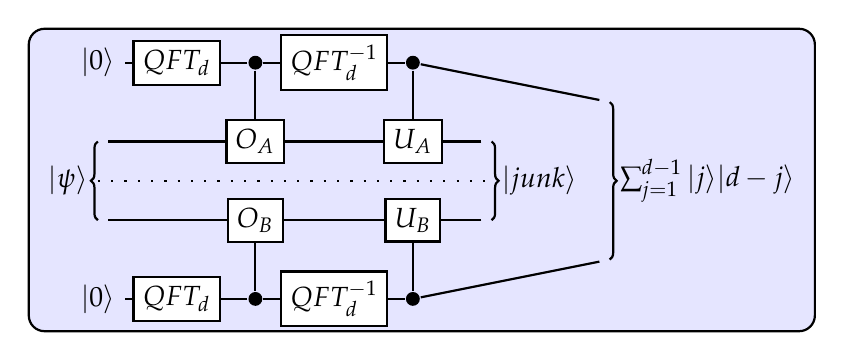
\begin{tikzpicture}[thick]
        %
        % `operator' will only be used by Hadamard (H) gates here.
        % `phase' is used for controlled phase gates (dots).
        % `surround' is used for the background box.
        \tikzstyle{operator} = [draw,fill=white,minimum size=1.5em] 
        \tikzstyle{phase} = [fill,shape=circle,minimum size=5pt,inner sep=0pt]
        \tikzstyle{surround} = [fill=blue!10,thick,draw=black,rounded corners=2mm]
        %
        % Bracket
        \draw[decorate,decoration={brace,mirror},thick] (0,-1) to
    	node[midway,left] (bracket1) {$\ket{\psi}$}
    	(0,-2);
        % Qubits
        \node at (0,0) (q1) {$\ket{0}$};
        \node at (0,-1) (q2) {};
        \node at (0,-2) (q3) {};
        \node at (0,-3) (q4) {$\ket{0}$};
        %
        % Column 1
        \node[operator] (op11) at (1,0) {$QFT_d$} edge [-] (q1);
        \node[operator] (op14) at (1,-3) {$QFT_d$} edge [-] (q4);
        %
        % Column 3
        \node[phase] (phase11) at (2,0) {} edge [-] (op11);
	\node[operator] (op22) at (2,-1) {$O_A$} edge [-] (q2);
	\node[operator] (op23) at (2, -2) {$O_B$} edge[-] (q3);
        \node[phase] (phase14) at (2,-3) {} edge [-] (op14);
        \draw[-] (phase11) -- (op22);
        \draw[-] (phase14) -- (op23);
        %
        % Column 4
        \node[operator] (op31) at (3,0) {$QFT_d^{-1}$} edge [-] (phase11);
        \node[operator] (op34) at (3,-3) {$QFT_d^{-1}$} edge [-] (phase14);
        %
        % Column 5
        \node[phase] (phase21) at (4,0) {} edge [-] (op31);
	\node[operator] (op42) at (4,-1) {$U_A$} edge [-] (op22);
	\node[operator] (op43) at (4, -2) {$U_B$} edge[-] (op23);
        \node[phase] (phase24) at (4,-3) {} edge [-] (op34);
        \draw[-] (phase21) -- (op42);
        \draw[-] (phase24) -- (op43);
        %
        % Column 6
        \node (end2) at (5,-1) {} edge [-] (op42);
        \node (end3) at (5,-2) {} edge [-] (op43);
        %
        % Bracket
        \draw[decorate,decoration={brace},thick] (5,-1) to
    	node[midway,right] (bracket) {$\ket{junk}$}
    	(5,-2);
        %
        % Column 7
        \node (end1) at (6.5,-0.5) {} edge [-] (phase21);
        \node (end4) at (6.5,-2.5) {} edge [-] (phase24);
        % Dashed line
        \draw[loosely dotted] (0,-1.5) -- (5,-1.5);
        % Bracket
        \draw[decorate,decoration={brace},thick,] (6.5,-0.5) to
    	node[midway,right] (bracket2) {$\sum_{j=1}^{d-1}\ket{j}\ket{d-j}$}
    	(6.5,-2.5);
        %
        % Background Box
        \begin{pgfonlayer}{background} 
        \node[surround] (background) [fit = (q1) (op14) (bracket1)(bracket2)] {};
        \end{pgfonlayer}
        %
        \end{tikzpicture}
	\caption{The isometries $\Phi_A$ and $\Phi_B$.}
\end{figure}
The isometry has the following steps:
\begin{enumerate}
	\item Append control register $\ket{0}_{A'}$ on Alice's side and $\ket{0}_{B'}$ on Bob's side;
	\item Apply Quantum Fourier Transform ($QFT_d$) to Alice and Bob's control registers;
	\item Apply Controlled-$O_{A/B}$ operations (i.e. if the control register is in state $\ket{k}_{A'/ B'}$, apply
	$O_{A/B}^k$.);
	\item Apply inverse Quantum Fourier Transform ($QFT_d^{-1}$) to the control registers;
	\item Apply Controlled-$U_{A/B}$ operations (i.e. If Alice's control register is in state $\ket{j}$, she applies
	$U_A^{\log_r (d-j)}$. If Bob's control register is in state $\ket{j}$, he applies $(U_B\ct)^{\log_r j}$).
\end{enumerate}
In order to show the isometry works, the key relations that we use are
\begin{align}
	&\ket{\psi} \appd{O(d^2 r^{1/4} \ep^{1/16})}\ket{\psi'} = \sum_{j=1}^{d-1} (U_A\ct U_B\ct)^{\log_r j} \ket{\psi_1},\\
	&O_A \ket{\psi_1} \appd{O(d\sr \ep^{1/8})} \omega_d^{-1} \ket{\psi_1},\\
	&O_B\ket{\psi_1} \appd{O(d \sr \ep^{1/8})} \omega_d \ket{\psi_1},\\
	&O_A(U_A\ct)^{\log_r j} \ket{\psi_1} \appd{O(d \sr \ep^{1/8})}\omega_d^{-r^j}  (U_A\ct)^j \ket{\psi_1}\\
	&O_B(U_A\ct)^{\log_r j} \ket{\psi_1} \appd{O(d \sr \ep^{1/8})}\omega_d^{r^j}  (U_A\ct)^j \ket{\psi_1}\
\end{align}
The result of this section is summarized in the theorem below.
\begin{theorem}
	Let $\Phi_A \x \Phi_B$ be the isometry defined above, then there exists a state $\ket{junk}$
	such that $\norm{\ket{junk}} \appd{O(r\se)} 1$ and 
	\begin{align}
		&\Phi_A \x \Phi_B (\ket{\psi}) \appd{O(d^2 r^{1/4} \ep^{1/16})} \ket{junk} \x \frac{1}{\sqrt{d-1}}\sum_{j=1}^{d-1} \ket{d-j}_{A'}\ket{j}_{B'}\\
		&\Phi_A \x \Phi_B (O_A\ket{\psi}) \appd{O(d^2 r^{1/4} \ep^{1/16})} \ket{junk} \x 
		\frac{1}{\sqrt{d-1}}\sum_{j=1}^{d-1} \omega_d^{d-j}\ket{d-j}_{A'}\ket{j}_{B'} \\
		&\Phi_A \x \Phi_B (O_B\ket{\psi}) \appd{O(d^2 r^{1/4} \ep^{1/16})} \ket{junk} \x 
		\frac{1}{\sqrt{d-1}}\sum_{j=1}^{d-1} \omega_d^{j}\ket{d-j}_{A'}\ket{j}_{B'}\\
		&\Phi_A \x \Phi_B (U_A\ket{\psi}) \appd{O(d^2 r^{1/4} \ep^{1/16})} \ket{junk} \x 
		\frac{1}{\sqrt{d-1}}\sum_{j=1}^{d-1} \ket{d-j/r}_{A'}\ket{j}_{B'} \\
		&\Phi_A \x \Phi_B (U_B\ket{\psi}) \appd{O(d^2 r^{1/4} \ep^{1/16})} \ket{junk} \x 
		\frac{1}{\sqrt{d-1}}\sum_{j=1}^{d-1} \ket{d-j}_{A'}\ket{j/r}_{B'}.
	\end{align}
\end{theorem}
\begin{proof}
Since $ \Phi_A \x \Phi_B (\ket{\psi}) \appd{O(d^2 r^{1/4} \ep^{1/16})}  \Phi_A \x \Phi_B (\ket{\psi'})$,  
we will focus on how the isometry evolves $\ket{\psi'}$.
The evolution is summarized below.
	\begin{align}
		& \sum_{j=1}^{d-1} (U_A\ct U_B\ct)^{\log_r j} \ket{\psi_1} \ket{0}_{A'}\ket{0}_{B'}\\
		\xrightarrow[]{QFT_d}& \frac{1}{d}\sum_{k_1,k_2 = 0}^{d-1} \sum_{j=1}^{d-1} (U_A\ct U_B\ct)^{\log_r j}  \ket{\psi_1}\ket{k_1}_{A'}\ket{k_2}_{B'}\\
		\xrightarrow[]{\text{Controlled-}O_{A/B}}& \frac{1}{d}\sum_{k_1,k_2 = 0}^{d-1} \sum_{j=1}^{d-1} O_A^{k_1}(U_A\ct)^{\log_r j} O_B^{k_2}(U_B\ct)^{\log_r j}
		\ket{\psi_1} \ket{k_1}_{A'}\ket{k_2}_{B'}\\
		\appd{O(d^2 \sr \ep^{1/8})}&\frac{1}{d} \sum_{k_1,k_2 = 0}^{d-1} \sum_{j=1}^{d-1} (U_A\ct U_B\ct)^{\log_r j}\omega_d^{(k_2-k_1)j}\ket{\psi_1} \ket{k_1}_{A'}\ket{k_2}_{B'}\\
		\xrightarrow[]{QFT_d^{-1}} &\frac{1}{d^2}\sum_{l_1,l_2 = 0}^{d-1}\sum_{j=1}^{d-1} (U_A\ct U_B\ct)^{\log_r j} 
		\omega_d^{k_1(d-j-l_1)}\omega_d^{k_2(j-l_2)}\ket{\psi_1} \ket{l_1}_{A'}\ket{l_2}_{B'}\\
		= &\sum_{j=1}^{d-1}(U_A\ct U_B\ct)^{\log_r j} \ket{\psi_1} \ket{d-j}_{A'}\ket{j}_{B'} \\
		\xrightarrow[]{\text{Controlled-}U_{A/B}}& \sum_{j=1}^{d-1} U_A^{\log_r j} (U_A\ct)^{\log_r j} U_B^{\log_r j} (U_B\ct)^{\log_r j} \ket{\psi_1} \ket{d-j}_{A'}\ket{j}_{B'}\\
		=&\ket{\psi_1} \x \sum_{j=1}^{d-1} \ket{d-j}_{A'}\ket{j}_{B'},
	\end{align}
So we define 
\begin{align}
	\ket{junk} = \sqrt{d-1}\ket{\psi_1},
\end{align}
such that 
\begin{align}
	\Phi_A\x\Phi_B(\ket{\psi}) \appd{O(d^2 r^{1/4} \ep^{1/16})} \ket{junk} \x \frac{1}{\sqrt{d-1}}\sum_{j=1}^{d-1} \ket{d-j}_{A'}\ket{j}_{B'}.
\end{align}
Since $\norm{\ket{\psi_1}}^2 \appd{O(r \se)} 1/(d-1)$, we know $\norm{\ket{junk}} \appd{O(r\se)} 1$.
	
If the initial state is $O_A\ket{\psi}$, we first use the fact that 
$ \Phi_A \x \Phi_B (O_A\ket{\psi}) \appd{O(d^2 r^{1/4} \ep^{1/16})}  \Phi_A \x \Phi_B (O_A\ket{\psi'})$, 
and then we calculate $\Phi_A \x \Phi_B (O_A\ket{\psi'})$.
\begin{align}
	O_A \ket{\psi'} \ket{0}_{A'}\ket{0}_{B'} =&  
		\sum_{j=1}^{d-1} O_A(U_A\ct U_B\ct)^{\log_r j}\ket{\psi_1}\ket{0}_{A'}\ket{0}_{B'}\\
		\appd{O(d^2 \sr \ep^{1/8})}&\sum_{j=1}^{d-1}(U_A\ct U_B\ct)^{\log_r j} \omega_d^{-j} \ket{\psi_1} \ket{0}_{A'}\ket{0}_{B'}\\
		\xrightarrow[]{QFT_d} &\frac{1}{d}\sum_{j=1}^{d-1} \sum_{k_1,k_2 = 0}^{d-1}(U_A\ct U_B\ct)^{\log_r j} \omega_d^{-j} 
		\ket{\psi_1}\ket{k_1}_{A'}\ket{k_2}_{B'}\\
		\xrightarrow[]{\text{Controlled-}O_{A/B}}&\frac{1}{d}\sum_{j=1}^{d-1}\sum_{k_1,k_2 = 0}^{d-1} 
		 O_A^{k_1}(U_A\ct)^{\log_r j} O_B^{k_2}(U_B\ct)^{\log_r j} \omega_d^{-j} \ket{\psi_1} \ket{k_1}_{A'}\ket{k_2}_{B'}\\
		\appd{O(d^2 \sr \ep^{1/8})}& \frac{1}{d}\sum_{k_1,k_2 = 0}^{d-1} \sum_{j=1}^{d-1} (U_A\ct U_B\ct)^{\log_r j}
		\omega_d^{-j}\omega_d^{(k_2-k_1)j}\ket{\psi_1}
		 \ket{k_1}_{A'}\ket{k_2}_{B'}\\
		\xrightarrow[]{QFT_d^{-1}}& \sum_{j=1}^{d-1}  (U_A\ct U_B\ct)^{\log_r j}  
		\omega_d^{d-j}\ket{\psi_1} \ket{d-j}_{A'}\ket{j}_{B'}\\
		\xrightarrow[]{\text{Controlled-}U_{A/B}}&   \sqrt{d-1} \ket{\psi_1} \x  
		\frac{1}{\sqrt{d-1}}\sum_{j=1}^{d-1} \omega_d^{d-j}\ket{d-j}_{A'}\ket{j}_{B'}.
\end{align}
The analysis for $\Phi_A\x\Phi_B(O_B \ket{\psi})$ is very similar.

If the initial state is $U_A\ket{\psi}$, we first use the fact that 
$ \Phi_A \x \Phi_B (U_A\ket{\psi}) \appd{O(d^2 r^{1/4} \ep^{1/16})}  \Phi_A \x \Phi_B (U_A\ket{\psi'})$, 
and then we calculate $\Phi_A \x \Phi_B U_A\ket{\psi'})$.
\begin{align}
	U_A \ket{\psi'} \ket{0}_{A'}\ket{0}_{B'} =&  
		\sum_{j=1}^{d-1} U_A(U_A\ct U_B\ct)^{\log_r j}\ket{\psi_1} \ket{0}_{A'}\ket{0}_{B'}\\
		=&\sum_{j=1}^{d-1}(U_A\ct)^{\log_r j-1}  (U_B\ct)^{\log_r j} \ket{\psi_1} \ket{0}_{A'}\ket{0}_{B'}\\
		\xrightarrow[]{QFT_d} &\frac{1}{d}\sum_{j=1}^{d-1} \sum_{k_1,k_2 = 0}^{d-1}(U_A\ct)^{\log_r j-1} (U_B\ct)^{\log_r j} \ket{\psi_1}  \ket{k_1}_{A'}\ket{k_2}_{B'}\\
		\xrightarrow[]{\text{Controlled-}O_{A/B}}&\frac{1}{d}\sum_{j=1}^{d-1}\sum_{k_1,k_2 = 0}^{d-1} 
		 O_A^{k_1}(U_A\ct)^{\log_r j-1} O_B^{k_2}(U_B\ct)^{\log_r j} \ket{\psi_1} \ket{k_1}_{A'}\ket{k_2}_{B'}\\
		\appd{O(d^2 \sr \ep^{1/8})}& \frac{1}{d}\sum_{k_1,k_2 = 0}^{d-1} \sum_{j=1}^{d-1} (U_A\ct)^{\log_r j-1} (U_B\ct)^{\log_r j}
		\omega_d^{k_2j-k_1j/r}\ket{\psi_1}
		 \ket{k_1}_{A'}\ket{k_2}_{B'}\\
		\xrightarrow[]{QFT_d^{-1}}& \sum_{j=1}^{d-1}  (U_A\ct)^{\log_r j-1} (U_B\ct)^{\log_r j}  
		\ket{\psi_1} \ket{d-j/r}_{A'}\ket{j}_{B'}\\
		\xrightarrow[]{\text{Controlled-}U_{A/B}}& \ket{junk} \x  
		\frac{1}{\sqrt{d-1}} \sum_{j=1}^{d-1} \ket{d-j/r}_{A'}\ket{j}_{B'}.
\end{align}
The analysis for $\Phi_A\x\Phi_B(U_B \ket{\psi})$ is very similar.
\end{proof}
%It means that $(U_A\ct)(U_B\ct)^j \ket{\psi_1} \in \spn(\supp(\ket{\psi}))$ for all $j \in [d-1]$,
%and so is $\ket{\psi'}$.
%\hl{[TODO] show that $\ket{\psi'}$ is obtained from $\ket{\psi}$ by local isometries.}


%%------------------------------------------------------------------------
%\subsection{The single value test}
%%------------------------------------------------------------------------
%By the following test, we want to make sure that $B_1B_2$ has eigenvalue $1$.
%The key observation is that $B_1B_2\ket{psi} = \ket{\psi}$ implies that 
%\begin{align}
%	\ket{\psi} = B_1\ket{\psi} = B_2 \ket{\psi}.
%\end{align}
%Alice and Bob will each get a symbol $x$,$y \in \{ 0, 1, \ast\}$ respectively and they answer with $a,b \in \{0,1,\diamond,\perp\}$. 
%The scoring rules are
%\begin{itemize}
%	\item \textbf{Case 1:} $x = y = \ast$, Alice and Bob should answer with $a, b \in \{\diamond, \perp\}$ and 
%	they score only if $a = b$;
%	\item \textbf{Case 2a:} $x =\ast$ and $y = 1$,  when Alice answer $\diamond$, Bob should answer $0$, when 
%	Alice answer$\perp$ all answers of Bob are accepted;
%	\item \textbf{Case 2b:} $x = \ast$ and $y = 2$,  when Alice answer $\diamond$, Bob should answer $0$, when 
%	Alice answer$\perp$ all answers of Bob are accepted.
%\end{itemize}
%
%The ideal strategy has projective measurement 
%\begin{align}
%&A_\ast^\diamond = B_\ast^\diamond= \ketbra{u_0}{u_0}, 
%&A_\ast^\perp = B_\ast^\perp = \1 - \ketbra{u_0}{u_0},
%\end{align}
%and Bob will reuse $B_1$ $B_2$ from his strategy to win the linear system game.
%The shared state is 
%\begin{align}
%	\ket{\psi} = \frac{1}{d} \sum_{i \in [d]} \ket{u_i}\ket{u_i}.
%\end{align}
%So in the ideal correlation, we have
%\begin{align}
%&P(\diamond \diamond| \ast \ast) = \bra{\psi} A_\ast^\diamond \otimes  B_\ast^\diamond \ket{\psi} = \frac{1}{d}\\
%	&P(\perp \perp| \ast \ast) = \bra{\psi} A_\ast^\perp \otimes B_\ast^\perp \ket{\psi} = \frac{d-1}{d}\\
%	&P(\diamond \perp| \ast \ast) = \bra{\psi} A_\ast^\diamond \otimes B_\ast^\perp \ket{\psi} = 0\\
%	&P(\perp \diamond| \ast \ast) = \bra{\psi} A_\ast^\perp \otimes B_\ast^\diamond \ket{\psi} = 0\\
%	&P(\diamond 0|\ast 1) = \bra{\psi} A_\ast^\diamond \otimes  B_1^0 \ket{\psi} = \frac{1}{d}\\
%	&P(\diamond 0|\ast 2) = \bra{\psi} A_\ast^\diamond \otimes  B_2^0 \ket{\psi} = \frac{1}{d}
%\end{align}
%By the marginal distribution we know that $\| A_\ast^\diamond \ket{\psi}\| = \frac{1}{\sqrt{d}}$.
%From the condition that $P(\diamond 0|\ast 1) = 1/d$, we know
%\begin{align}
%	\frac{  \bra{\psi} A_\ast^\diamond  B_1^0 \ket{\psi}}{\| A_\ast^\diamond \ket{\psi}\|^2} = 1,
%\end{align}
%which implies that 
%\begin{align}
% B_1^0 \frac{A_\ast^\diamond \ket{\psi}}{\| A_\ast^\diamond \ket{\psi}\|} = \frac{A_\ast^\diamond \ket{\psi}}{\| A_\ast^\diamond \ket{\psi}\|}.
%\end{align}
%With similar reasoning, we get
%\begin{align}
% B_2^0 \frac{A_\ast^\diamond \ket{\psi}}{\| A_\ast^\diamond \ket{\psi}\|} = \frac{A_\ast^\diamond \ket{\psi}}{\| A_\ast^\diamond \ket{\psi}\|}.
%\end{align}
%Hence $ \frac{A_\ast^\diamond \ket{\psi}}{\| A_\ast^\diamond \ket{\psi}\|} $ is in the intersection of $\supp(B_1^0)$ and $\supp(B_2^0)$.
%Since $\supp(B_x^0)$ and $\supp(B_x^1)$ are disjoint, we know
%\begin{align}
%	B_x  \frac{A_\ast^\diamond \ket{\psi}}{\| A_\ast^\diamond \ket{\psi}\|}  =  \frac{A_\ast^\diamond \ket{\psi}}{\| A_\ast^\diamond \ket{\psi}\|} 
%\end{align}
%for $x = 1,2$.
%Therefor, we know $ \frac{A_\ast^\diamond \ket{\psi}}{\| A_\ast^\diamond \ket{\psi}\|} $ is an eigenvector of $B_1B_2$ with eigenvalue $1$ because
%\begin{align}
%	B_1B_2 \frac{A_\ast^\diamond \ket{\psi}}{\| A_\ast^\diamond \ket{\psi}\|} = B_1 \frac{A_\ast^\diamond \ket{\psi}}{\| A_\ast^\diamond \ket{\psi}\|} =  \frac{A_\ast^\diamond \ket{\psi}}{\| A_\ast^\diamond \ket{\psi}\|}.
%\end{align}
%In the later section, when we apply this test to make sure some unitary $U$ has eigenvalue $1$ with one-dimensional eigen-space, we denote the test by $\SVT_U$.
%====================================
\section{The new game} 
\label{sec:main}
%=====================================

Alice receives $x \in \{1,\dots m_r+3 \}$ and Bob receives
$y \in \{1,\dots,n_r+1\}$. We follow the previous structure by first give intuition about how they should
behave in this game. The correlation can be easily extracted from the behaviour list below.
\begin{itemize}
	\item When $x \in \{1,\dots m_r\}$ and $y \in \{1, \dots n_r\}$, they should win the 
	linear system game $LS_r$ perfectly;
	\item when $x \in \{m_r+1, m_r+2, m_r+3\}$ and $y \in \{1, 2, n_r+1\}$, they should follow the
	optimal correlation of the test $\CHSH_X$, where 
	\begin{align}
		&\ast_A = m_r+1, \quad 1_A = m_r+2,\quad 2_A = m_r+3,\\
		&\ast_B = n_r+1,\quad 1_B = 1, \quad 2_A = 2,
	\end{align}
	are the inputs for the game $\CHSH_X$
	(The intuition behind is that $B_1B_2 = X$.);
	\item otherwise, their behaviour is irrelevant.
\end{itemize}
Note that the dimension $d$ is defined in the rules of $\CHSH_X$.
Next we are going to prove that the strategy winning this game optimally can self-test $d$-dimensional EPR pair and 
$d$-dimensional $\sigma_x$ and $\sigma_z$.
%In the ideal case, Alice and Bob share state $\ket{\psi} = \frac{1}{d-1} \sum_{i=1}^{d-1}\ket{ii}$.
%They first append control register $\ket{0}$ to their own share of $\ket{\psi}$.
%then apply $QFT_d$ to the control register, which evolves the state as
%\begin{align}
%	\ket{\psi} \ket{0}_A\ket{0}_B \to \frac{1}{d} \sum_{k_1, k_2 =  0}^{d-1} \ket{\psi}\ket{k_1}_A\ket{k_2}_B.
%\end{align}
%Controlled by the control register $X_A^{k_1}$ and $X_B^{k_2}$ are applied and the state becomes
%\begin{align}
%	\frac{1}{d} \sum_{k_1, k_2 =  0}^{d-1} \ket{\psi}\ket{k_1}_A\ket{k_2}_B \to
%	\frac{1}{d} \sum_{k_1, k_2 =  0}^{d-1} X_A^{k_1} X_B^{k_2}\ket{\psi}\ket{k_1}_A\ket{k_2}_B.
%\end{align}
%In the ideal case $X_A = X_B = \sum_{i=1}^{d-1} \omega_d^i \ketbra{i}{i}$, then
%\begin{align}
%	X_A^{k_1} X_B^{k_2}\ket{\psi} &= 
%	\sum_{i_1,i_2 = 1}^{d-1} \omega_d^{i_1k_1+i_2k_2} \ketbra{i_1}{i_1}_A \x\ketbra{i_2}{i_2}_B \ket{\psi}\\
%	&=\frac{1}{\sqrt{d-1}}  \sum_{i_1 = 1}^{d-1} \omega_d^{i_1(k_1+k_2)} \ket{i_1i_1}.
%\end{align}
%Then they apply inverse $QFT_d$ to the control register, the shared state becomes
%\begin{align}
%	&\frac{1}{d\sqrt{d-1}} \sum_{k_1, k_2 =  0}^{d-1}\sum_{i_1 = 1}^{d-1} \omega_d^{i_1(k_1+k_2)} \ket{i_1i_1}\\
%	\to& \frac{1}{d^2\sqrt{d-1}} \sum_{k_1, k_2,l_1,l_2 =  0}^{d-1}
%	\sum_{i_1 = 1}^{d-1}\omega_d^{k_1(i_1-l_1)}\omega_d^{k_2(i_1-l_2)} \ket{i_1i_1} \ket{l_1}_A\ket{l_2}_B\\
%	=& \frac{1}{\sqrt{d-1}} \sum_{i = 1}^{d-1} \ket{i i} \ket{i}_A\ket{i}_B.
%\end{align}
%In the last step $U_A^{k_i}$ and $U_B^{k_i}$ are applied when the control register is in the state 
%$\ket{i}_{A/B}$, where $k_i$ satisfies the condition that $r^{k_i} \equiv i \pmod{d}$, and the state 
%becomes
%\begin{align}
%	\frac{1}{\sqrt{d-1}} \sum_{i = 1}^{d-1} \ket{i i} \ket{i}_A\ket{i}_B \to &
%	\frac{1}{\sqrt{d-1}} \sum_{i = 1}^{d-1}U_A^{k_i} U_B^{k_i} \ket{i i} \ket{i}_A \ket{i}_B\\
%	= & \frac{1}{\sqrt{d-1}} \sum_{i = 1}^{d-1} \ket{i (r^{-1})^k}\ket{i (r^{-1})^k}\ket{i}_A \ket{i}_B \\
%	= & \ket{11} \x \frac{1}{\sqrt{d-1}} \sum_{i = 1}^{d-1}\ket{i}_A \ket{i}_B.
%\end{align}
%
%If we want to generalize the isometry, we need ways to deconstruct $X_{A/B}$ as 
%a linear combination of projectors. Recall that in the ideal strategy $A_{m_r+2}^0 = \ketbra{1}{1}$,
%so we can write 
%\begin{align}
%	X_A = \sum_{i=1}^{d-1} \omega_d^{2^{k_i}} U_A^{k_i} A_{m_r+2}^0 (U_A\ct)^{k_i}
%	= \sum_{i=1}^{d-1} \omega_d^i U_A^{k_i} A_{m_r+2}^0 (U_A\ct)^{k_i}.
%\end{align}
%On Bob's side, we use the fact that 
%\begin{align}
%B' := B_{n_r+1}^\diamond \frac{B_1^0 + B_2^0}{2\cos(\pi/2d)} B_{n_r+1}^\diamond = \ketbra{1}{1},
%\end{align}
%and write
%\begin{align}
%	X_B =\sum_{i=1}^{d-1} \omega_d^i U_B^{k_i} B' (U_B\ct)^{k_i}.
%\end{align}
%So we need to show that for all $i=1 \dots d-1$,
%\begin{align}
%	U_B^{k_i} B' (U_B\ct)^{k_i} \ket{\psi} = U_A^{k_i} A_{m_r+2}^0 (U_A\ct)^{k_i} \ket{\psi}.
%\end{align}
%Intuitively, Bob's operation can be moved to Alice's side.
%We also need to show that, for $i \neq j$, 
%\begin{align}
%	U_A^{k_i} A_{m_r+2}^0 (U_A\ct)^{k_i} U_A^{k_j} A_{m_r+2}^0 (U_A\ct)^{k_j} \ket{\psi} = 0.
%\end{align}
%Otherwise, we need different way to represent the eigen-structure of $X_{A/B}$.

%-----------------------------------------------
\subsection{Proof Sketch}
%-----------------------------------------------
Now we examine the implications of Alice and Bob winning the linear constraint game perfectly.
By Lemma~$4.3$ of \cite{coladan2017}, we can extract an operator solution from the perfect winning strategy 
of the linear system game: 
For each variable $\{ x_i \}_{i=1}^n$, Alice and Bob has operators $A_i$ and $B_i$ respectively.
The condition that they agree with assignment to variables means that 
\begin{align}
	\bra{\psi} A_i \otimes \overline{B_i} \ket{\psi} \geq 1 - O(r\epsilon) \Rightarrow 
	A_i \otimes \overline{B_i} \ket{\psi} \appd{O(\sqrt{r\epsilon})} \ket{\psi}
\end{align}
and the condition that Alice's assignments almost satisfy the constraint means that 
for each $i \in [m_r]+1$,
\begin{align}
\bra{\psi} \Pi_{j:H(i,j) \neq 0} A_j \ket{\psi} \geq 1- m_r \epsilon,
\end{align}
which means that 
\begin{align}
	\Pi_{j:H(i,j) \neq 0} A_j \ket{\psi} \appd{\sqrt{r\epsilon}} \ket{\psi},
\end{align}
where we use the fact that $m_r \in O(r)$.
Following the steps of the embedding of $x_3x_4x_1x_2x_4x_3 = (x_1x_2)^r$ into the linear system game,
we can conclude that 
\begin{align}
	A_3A_4 A_1A_2 (A_3A_4)^\dagger \ket{\psi}\appd{O(r\sqrt{r\epsilon})} (A_1A_2)^r \ket{\psi}.
\end{align}
For simplicity, we define $X_A = A_1A_2$ and $U_A=A_3A_4$ such that
the condition is equivalent to
\begin{align}
	\label{eq:ux_relation}
	U_AX_AU_A^\dagger \ket{\psi} \appd{O(r\sqrt{r\epsilon})} X_A^r \ket{\psi}.
\end{align}
Since the relation $ux^{-1}u^{-1} = x^{-r}$ is also embedded in $LS_r$, we know
\begin{align}
	U_AX_A\ct U_A\ct \ket{\psi}\appd{O(r\sqrt{r\epsilon})} (X_A\ct)^r \ket{\psi}.
\end{align}
Combining the two equations above, we get 
\begin{align}
	U_A(X_A+X_A\ct)U_A\ct \ket{\psi} \appd{O(r\sqrt{r\epsilon})} [(X_A\ct)^r+(X_A)^r] \ket{\psi},\\
	U_B(X_B+X_B\ct)U_B\ct \ket{\psi} \appd{O(r\sqrt{r\epsilon})} [(X_B\ct)^r+(X_B)^r] \ket{\psi}.
\end{align}
We will come back to the implication of this condition later.

Next we look at the implication of winning the $\CHSH_{X}$ game almost optimally.
It means that the quantum strategy $\{ \{A_{m_r+2}^a, A_{m_r+3}^a\}_{a=0,1},\{B_1^b,  B_2^b\}_{b=0,1}, A_{m_r+1}^\diamond B_{n_r+1}^\diamond \ket{\psi}\}$ violates the $\I_\alpha$ almost optimally, i.e., $\ip{I_\alpha} = 2\sqrt{1+a^2}-\epsilon$. 
From \cref{prop:2d-subspace}, we know that 
\begin{align}
	[(B_1B_2)^r + (B_2B_1)^r] B_{n_r+1}^\diamond \ket{\psi} \appd{O(2^{r-1}\sqrt{\epsilon})} 
	2\cos(\frac{2r\pi}{d}) B_{n_r+1}^\diamond \ket{\psi},
\end{align}
Or equivalently,
\begin{align}
\label{eq:b_to_cos}
	[X_B^r + (X_B\ct)^r] B_{n_r+1}^\diamond \ket{\psi} \appd{O(2^{r-1}\sqrt{\epsilon})} 
	2\cos(\frac{2r\pi}{d}) B_{n_r+1}^\diamond \ket{\psi}.
\end{align}

In the next step, we would like to 
relate $U_B(X_B+X_B\ct)U_B\ct B_{n_r+1}^\diamond \ket{\psi}$ to $2\cos(\frac{2r\pi}{d}) B_{n_r+1}^\diamond \ket{\psi}$.
Since $\ket{\psi} = B_{n_r+1}^\diamond \ket{\psi} + B_{n_r+1}^\perp \ket{\psi}$, we start with
\begin{align*}
	&\norm{[U_B(X_B+X_B\ct)U_B\ct - ((X_B\ct)^r+(X_B)^r)]\ket{\psi}}^2\\
	= &\norm{[U_B(X_B+X_B\ct)U_B\ct - ((X_B\ct)^r+(X_B)^r)]B_{n_r+1}^\diamond \ket{\psi}\\
	&+ [U_B(X_B+X_B\ct)U_B\ct - ((X_B\ct)^r+(X_B)^r)]B_{n_r+1}^\perp \ket{\psi}}^2\\
	=&\norm{[U_B(X_B+X_B\ct)U_B\ct - ((X_B\ct)^r+(X_B)^r)]B_{n_r+1}^\diamond \ket{\psi}}^2 \\
	&+\norm{[U_B(X_B+X_B\ct)U_B\ct - ((X_B\ct)^r+(X_B)^r)]B_{n_r+1}^\perp \ket{\psi}}^2 \\
	&+\bra{\psi} B_{n_r+1}^\diamond [U_B(X_B+X_B\ct)U_B\ct - ((X_B\ct)^r+(X_B)^r)]^2 B_{n_r+1}^\perp \ket{\psi}\\
	&+\bra{\psi} B_{n_r+1}^\perp [U_B(X_B+X_B\ct)U_B\ct - ((X_B\ct)^r+(X_B)^r)]^2 B_{n_r+1}^\diamond \ket{\psi}
\end{align*}
Here, we use the following proposition to bound $\bra{\psi} B_{n_r+1}^\diamond [U_B(X_B+X_B\ct)U_B\ct - ((X_B\ct)^r+(X_B)^r)]^2 B_{n_r+1}^\perp \ket{\psi}$ and $\bra{\psi} B_{n_r+1}^\perp [U_B(X_B+X_B\ct)U_B\ct - ((X_B\ct)^r+(X_B)^r)]^2 B_{n_r+1}^\diamond \ket{\psi}$.
Going back to our target,
\begin{align}
	&\qquad\bra{\psi} B_{n_r+1}^\perp [U_B(X_B+X_B\ct)U_B\ct - ((X_B\ct)^r+(X_B)^r)]^2 B_{n_r+1}^\diamond \ket{\psi} \\
	&\appd{O(\sqrt{\epsilon})} \bra{\psi} B_{n_r+1}^\perp [U_B(X_B+X_B\ct)U_B\ct - ((X_B\ct)^r+(X_B)^r)]^2 A_{m_r+1}^\diamond \ket{\psi} \\
	&=\bra{\psi} A_{m_r+1}^\diamond B_{n_r+1}^\perp[U_B(X_B+X_B\ct)U_B\ct - ((X_B\ct)^r+(X_B)^r)]^2 \ket{\psi}\\
	&\appd{O(\sqrt{\epsilon})} \bra{\psi} B_{n_r+1}^\diamond B_{n_r+1}^\perp[U_B(X_B+X_B\ct)U_B\ct - ((X_B\ct)^r+(X_B)^r)]^2 \ket{\psi}\\
	&= 0.
\end{align}
With similar reasoning, we can prove that
\begin{align}
	|\bra{\psi} B_{n_r+1}^\diamond [U_B(X_B+X_B\ct)U_B\ct - ((X_B\ct)^r+(X_B)^r)]^2 B_{n_r+1}^\perp \ket{\psi}| = O(\sqrt{\epsilon}).
\end{align}	
Hence, we can conclude that 
\begin{align}
	O(r^3\epsilon) \geq &\norm{[(U_B(X_B+X_B\ct)U_B\ct) - ((X_B)^r + (X_B\ct)^r)](B_{n_r+1}^\diamond + B_{n_r+1}^\perp)\ket{\psi}}^2\\
	= &\norm{[(U_B(X_B+X_B\ct)U_B\ct) - ((X_B)^r + (X_B\ct)^r)]B_{n_r+1}^\diamond\ket{\psi}}^2\\
	&+ \norm{[(U_B(X_B+X_B\ct)U_B\ct) - ((X_B)^r + (X_B\ct)^r)]B_{n_r+1}^\perp\ket{\psi}}^2 +O(\sqrt{\epsilon})\\
	\geq &\norm{[(U_B(X_B+X_B\ct)U_B\ct) - ((X_B)^r + (X_B\ct)^r)]B_{n_r+1}^\diamond\ket{\psi}}^2 + O(\sqrt{\epsilon})
\end{align}
which means that 
\begin{align}
(U_B(X_B+X_B\ct)U_B\ct)B_{n_r+1}^\diamond \ket{\psi} \appd{O(r^{3/2} \epsilon^{1/4})}((X_B)^r + (X_B\ct)^r)]B_{n_r+1}^\diamond\ket{\psi}.
\end{align}
Juxtaposing the relation above with \cref{eq:b_to_cos}, we get
\begin{align}
	(U_B(X_B+X_B\ct)U_B\ct) B_{n_r+1}^\diamond \ket{\psi} 
	\appd{O(2^{r+1}\epsilon^{1/4})} \cos(\frac{2r\pi}{d}) B_{n_r+1}^\diamond\ket{\psi},
\end{align}
or equivalently,
\begin{align}
	(X_B + X_B\ct) U_B\ct B_{n_r+1}^\diamond \ket{\psi} \appd{O(2^{r+1}\epsilon^{1/4})}  
	2\cos(\frac{2r\pi}{d}) U_B\ct B_{n_r+1}^\diamond \ket{\psi}.
\end{align}
Intuitively, it says that $U_B\ct B_{n_r+1}^\diamond \ket{\psi}$ is close to an eigenvector of 
the Hermitian matrix $X_B +X_B\ct$ with eigenvalue $2\cos(\frac{2r\pi}{d})$.
Comparing it with the fact that
\begin{align}
(X_B + X_B\ct) B_{n_r+1}^\diamond \ket{\psi} \appd{O(\sqrt{\epsilon})}  
	2\cos(\frac{2\pi}{d}) B_{n_r+1}^\diamond \ket{\psi},
\end{align}
we would like to draw the conclusion that $B_{n_r+1}^\diamond \ket{\psi}$ is 
close to orthogonal to $U_B\ct B_{n_r+1}^\diamond \ket{\psi}$
by the following proposition.
Following \cref{prop:orthog} and the 
and the fact that $(X_B + X_B\ct)$ is Hermitian, we can conclude that
\begin{align}
\bra{\psi}B_{n_r+1}^\diamond U_B\ct B_{n_r+1}^\diamond \ket{\psi} = O(\frac{2^{r+1}\epsilon^{1/4}}{\cos(2\pi/d) - \cos(2r\pi/d)}).
\end{align}
%It means that there exists isometris $V_A$ on Alice side and $V_B$ on Bob's side such that 
%\begin{align}
%	&(V_A\otimes V_B)  \frac{A_\ast^\diamond \otimes B_\ast^\diamond \ket{\psi}}{\|A_\ast^\diamond \otimes B_\ast^\diamond \ket{\psi}\|}
%	= \frac{1}{\sqrt{2}} (\ket{00} + \ket{11}) \otimes \ket{extra} \\
%	&(V_A\otimes V_B) \frac{B_1 + B_2}{2\cos(\pi/2d)} \frac{A_\ast^\diamond \otimes B_\ast^\diamond \ket{\psi}}{\|A_\ast^\diamond \otimes B_\ast^\diamond \ket{\psi}\|}
%	= (\1 \otimes \sigma_z)\frac{1}{\sqrt{2}} (\ket{00} + \ket{11}) \otimes \ket{extra}\\
%	&(V_A\otimes V_B) \frac{B_1 - B_2}{-2\sin(\pi/2d)} \frac{A_\ast^\diamond \otimes B_\ast^\diamond \ket{\psi}}{\|A_\ast^\diamond \otimes B_\ast^\diamond \ket{\psi}\|}
%	= (\1 \otimes \sigma_x)\frac{1}{\sqrt{2}} (\ket{00} + \ket{11}) \otimes \ket{extra}.
%\end{align}
%Suppose $A_\ast^\diamond$ measures states $\ket{u_0}$ and $\ket{u_1}$. Then we know
%\begin{align}
%	&(B_1 + B_2) \ket{u_0} = 2\cos(\pi/2d) \ket{u_0} \\
%	&(B_1 + B_2) \ket{u_1} = -2\cos(\pi/2d) \ket{u_1}\\
%	&(B_1 - B_2) \ket{u_0} = -2\sin(\pi/2d) \ket{u_1} \\
%	&(B_1 - B_2) \ket{u_1} = -2\sin(\pi/2d) \ket{u_0}
%\end{align}
%which implies that 
%\begin{align*}
%	B_1 \ket{u_0} &= \cos(\pi/2d) \ket{u_0} - \sin(\pi/2d) \ket{u_1} \\
%	B_2 \ket{u_0} &= \cos(\pi/2d) \ket{u_0} + \sin(\pi/2d) \ket{u_1} \\
%	B_1 \ket{u_1} &= -\sin(\pi/2d) \ket{u_0}-\cos(\pi/2d) \ket{u_1} \\
%	B_2 \ket{u_1} &= \sin(\pi/2d) \ket{u_0}-\cos(\pi/2d) \ket{u_1} \\
%	B_1B_2 \ket{u_0} &= \cos(\pi/2d) B_1\ket{u_0} + \sin(\pi/2d) B_1\ket{u_1} \\
%	&=\cos(\pi/2d) (\cos(\pi/2d) \ket{u_0} - \sin(\pi/2d) \ket{u_1}) -\sin(\pi/2d)(\sin(\pi/2d) \ket{u_0} + \cos(\pi/2d)\ket{u_1})\\
%	&=\cos(\pi/d) \ket{u_0} -\sin(\pi/d) \ket{u_1}\\
%	B_1B_2\ket{u_1} &= \sin(\pi/2d) B_1\ket{u_0}-\cos(\pi/2d) B_1\ket{u_1} \\
%	&= \sin(\pi/2d) (\cos(\pi/2d) \ket{u_0} - \sin(\pi/2d) \ket{u_1}) + \cos(\pi/2d)(\sin(\pi/2d) \ket{u_0}+\cos(\pi/2d) \ket{u_1})\\
%	&= \sin(\pi/d)\ket{u_0} + \cos(\pi/d) \ket{u_1}.
%\end{align*}
%We can conclude that 
%\begin{align}
%	&B_1B_2(\ket{u_0} + i\ket{u_1}) = e^{i \frac{\pi}{d}} (\ket{u_0} + i\ket{u_1})\\
%	&B_1B_2(\ket{u_0} - i\ket{u_1}) = e^{-i \frac{\pi}{d}} (\ket{u_0} - i\ket{u_1}).
%\end{align}
%Define $\ket{x_1} = 1/\sqrt{2}(\ket{u_0} + i\ket{u_1})$, then it is the eigenvector of $X$ with eigenvalue $e^{i\pi/d} = \omega_d$.
%Similarly, define $\ket{x_{d-1}} = 1/\sqrt{2}(\ket{u_0} - i\ket{u_1})$ such that $X \ket{x_{d-1}} = \omega_d^{d-1}\ket{x_{d-1}}$.
%We know 
%\begin{align}
%	\tA_\ast^\diamond \ket{\tpsi} = \tA_\ast^\diamond \x \tB_\ast^\diamond \ket{\tpsi} = \frac{1}{\sqrt{d}} (\ket{u_0}\ket{u_0} + \ket{u_1}\ket{u_1}).
%\end{align}
%If we restrict to Alice's system, we get 
%\begin{align}
%	\Tr_B(\tA_\ast^\diamond \ketbra{\tpsi}{\tpsi} \tA_\ast^\diamond) =\tA_\ast^\diamond \rho_A \tA_\ast^\diamond = 
% \frac{1}{d} \ketbra{u_0}{u_0} + \ketbra{u_1}{u_1} = \frac{1}{d} \tA_\ast^\diamond.
%\end{align}
%\hl{Hence $\rho_A$ acts as $\1$ on $\supp(\tA_\ast^\diamond)$.}
%We also know that there exists local unitary $U_A$ such that 
%\begin{align}
%U_A \tA_\ast^\diamond U_A^\dagger = \ketbra{x_1}{x_1}+\ketbra{x_{d-1}}{x_{d-1}}
%\end{align}
%and 
%\begin{align}
%\Tr(\ketbra{x_1}{x_1} \rho_A)
%=\Tr(U_A \ketbra{u_0}{u_0} U_A^\dagger \rho_A) 
%= \frac{1}{d} \Tr(U_A\ketbra{u_0}{u_0} U_A^\dagger) 
%= \frac{1}{d},
%\end{align}
%and similarly $\Tr( \ketbra{x_{d-1}}{x_{d-1}}\rho_A) = 1/d$.
%
%Based on \cref{eq:sim}, we know
%\begin{align}
%\label{eq:ladder}
% XU^\dagger \ket{x_1} = U^\dagger X^2 \ket{x_1} = \omega_d^2 U^\dagger \ket{x_1},
%\end{align}
%so $U^\dagger \ket{x_1}$ is an eigenvector of $X$ with eigenvalue $\omega_d^2$.
%By induction, we know $X (U^\dagger)^i \ket{x_1} = \omega_d^{2^i} (U^\dagger)^i\ket{x_1}$. 
%From the set $\{(U^\dagger)^i \ket{x_1}\}_{i=0}^{d-2}$, we can identify $\ket{x_i}$ for $1 \leq i \leq d-1$
%such that $X \ket{x_i} = \omega_d^i \ket{x_i}$.
%From the single value test, we know 
%\begin{align}
%	\tA_\triangle^\diamond \ket{\tpsi} = \tA_\triangle^\diamond \x \tB_\triangle^\diamond \ket{\tpsi} = \frac{1}{\sqrt{d}}
%	\ket{x_0}\ket{x_0}
%\end{align}
%where $X \ket{x_0} = \ket{x_0}$. Hence 
%\begin{align}
%	\tA_\triangle^\diamond  = \ketbra{x_0}{x_0}
%\end{align}
%and 
%\begin{align}
%	\tA_\triangle^\diamond \rho_A \tA_\triangle^\diamond = \frac{1}{d} \ketbra{x_0}{x_0} = \frac{1}{d} \tA_\triangle^\diamond.
%\end{align}
%
%The full eigen-decomposition of $X$ is
%\begin{align}
%	X = \sum_{i=0}^{d-1} \omega_d \ketbra{x_i}{x_i}.
%\end{align}
%\hl{[Can we get the full eigen-decomposition from the unitarity of $X$?]}
%If we substitute this eigen-decomposition into \cref{eq:sim}, we have 
%\begin{align}
%	\sum_{i=0}^{d-1} \omega_d^i \Tr( U\ketbra{x_i}{x_i}U^{-1} \rho_A) = \sum_{i=0}^{d-1} \omega_d^{2i} \Tr(\ketbra{x_i}{x_i}\rho_A),
%\end{align}
%or equivalently
%\begin{align}
%	\sum_{i=0}^{d-1} \omega_d^i \Tr\left[ \left(U\ketbra{x_i}{x_i}U^{-1}- \ketbra{x_{i/2}}{x_{i/2}}\right) \rho_A\right] =0.
%\end{align}
%Define $\alpha_i = \Tr\left[ \left(U\ketbra{x_i}{x_i}U^{-1}- \ketbra{x_{i/2}}{x_{i/2}}\right) \rho_A\right] \in [-1, 1] $.
%The fact that $\sum_{i=0}^{d-1} \alpha_i  \omega_d^i = 0$ implies that 
%$\alpha_i = 0$ or $\alpha_i = 1$ for all $i$.
%Let's look at $\alpha_2$, which is defined to be
%\begin{align}
%	 \alpha_2 = \Tr( U\ketbra{x_2}{x_2}U^{-1} \rho_A ) - \Tr(\ketbra{x_1}{x_1}\rho_A) 
%	 = \Tr( U\ketbra{x_2}{x_2}U^{-1} \rho_A ) - \frac{1}{d} 
%	 \leq 1 - \frac{1}{d},
%\end{align}
%so $\alpha_2 = 0$ and $\alpha_i = 0$ for all $i$.
%
%
%
%If we trace out Bob's system, we get 
%\begin{align}
%	&\Tr_B\left[ (U_A\x U_B)(\tA_\ast^\diamond) \ketbra{\tpsi}{\tpsi} (\tA_\ast^\diamond) (U_A\x U_B)^\dagger\right]\\
%	=& U_A \tA_\ast^\diamond \rho_A \tA_\ast^\diamond U_A^\dagger\\
%	=& \frac{1}{d}( \ketbra{x_1}{x_1} + \ketbra{x_{d-1}}{x_{d-1}})
%\end{align}
%where $U_A =U_B = \ketbra{x_1}{u_0} + \ketbra{x_{d-1}}{u_1}$ when their actions are restricted to 
%$\supp(\tA_\ast^\diamond)$.
%By \cref{eq:ladder}, we get 
%\begin{align}
%	U^\dagger U_A \tA_\ast^\diamond \rho_A \tA_\ast^\diamond U_A^\dagger U = \frac{1}{d}( \ketbra{x_2}{x_2} + \ketbra{x_{d-2}}{x_{d-2}})
%\end{align}
%So if we repeatedly conjugate $U_A \tA_\ast^\diamond \rho_A \tA_\ast^\diamond U_A^\dagger$ by $U^\dagger$ $d-1$ times and sum the equations up, we get 
%\begin{align}
%	\sum_{i=0}^{d-2} (U^\dagger)^i U_A \tA_\ast^\diamond \rho_A \tA_\ast^\diamond U_A^\dagger U^i
%	= \frac{2}{d} \sum_{i=1}^{d-1} \ketbra{x_i}{x_i}.
%\end{align}
%Note that here we used the fact that $d$ has primitive root $2$.
%
%
%From the single value test, we know 
%\begin{align}
%	\tA_\triangle^\diamond \ket{\tpsi} = \tA_\triangle^\diamond \x \tB_\triangle^\diamond \ket{\tpsi} = \frac{1}{\sqrt{d}}
%	\ket{x_0}\ket{x_0}
%\end{align}
%where $X \ket{x_0} = \ket{x_0}$.
%Again, we trace out Bob's system and get that
%\begin{align}
%	\tA_\triangle^\diamond \rho_A \tA_\triangle^\diamond = \frac{1}{d} \ketbra{x_0}{x_0}.
%\end{align}
%Define $V = A_\triangle^\diamond + \sum_{i=0}^{(d-1)/2} (U^\dagger)^i U_A \tA_\ast^\diamond$, we can check that 
%\begin{align}
%	V V^\dagger =A_\triangle^\diamond  + \sum_{i,j=0}^{(d-1)/2} (U^\dagger)^i U_A \tA_\ast^\diamond U_A^\dagger U^j
%\end{align}
%Moreover, 
%\begin{align}
%	&\Tr(\tA_\triangle^\diamond \rho_A \tA_\triangle^\diamond) + \sum_{i=0}^{(d-1)/2} \Tr[(U^\dagger)^i U_A \tA_\ast^\diamond \rho_A \tA_\ast^\diamond U_A^\dagger U^i] \\
%	=& \Tr(\tA_\triangle^\diamond \rho_A) + \sum_{i=0}^{(d-1)/2} \Tr[  \tA_\ast^\diamond U_A (U^\dagger)^{2i} U_A\tA_\ast^\diamond \rho_A] \\
%	=&1 \\
%	=& \Tr(\rho_A).
%\end{align}

%Define $\ket{x_1} = 1/\sqrt{2}(\ket{u_0} + i\ket{u_1})$, then it is the eigenvector of $B_1B_2$ with eigenvalue $e^{i\pi/d} = \omega_d$.
%Similarly, we define $\ket{x_{d-1}} = 1/\sqrt{2} (\ket{u_0} - i\ket{u_1})$ and it is the eigenvector of $B_1B_2$ with eigenvalue $\omega_d^{d-1}$.
%Moreover, from the self-testing derivation, we know 
%\begin{align}
% \|(\ketbra{x_1}{x_1} + \ketbra{x_{d-1}}{x_{d-1}})\ket{\psi}\|^2 = 2/d.
%\end{align}
%The condition that $B_1B_2 \sim (B_1B_2)^2$ implies that $\omega_d, \omega_d^2, \omega_d^4 \dots $ are all the eigenvalues of $B_1B_2$ and the eigen-space of each eigenvalue are of dimension $1$. 
%Since $2$ is a primitive root of $d$, we know $\omega_d^i = \omega_d^{2^{k_i}}$ for some $k_i$ and $i \in \{1,2 \dots, d-1\}$, or equivalently, $2^{k_i} \equiv i \pmod{d}$, which means that $B_1B_2$ is finite-dimensional and we have states $\ket{x_i}$ for $i = 1 \dots d-1$ such that 
%\begin{align}
%	B_1B_2 \ket{x_i} = \omega_d^i \ket{x_i}
%\end{align}
%and 
%\begin{align}
%	 \|(\sum_{i=1}^{d-1} \ketbra{x_i}{x_i})\ket{\psi}\|^2 = \frac{d-1}{d}.
%\end{align}
%
%The implication of the $\SVT_{\sigma_x}$ is that there exists state $\ket{x_0}$ such that 
%\begin{align}
%	B_1B_2 \ket{x_0} = \ket{x_0} \text{ and } \| \ketbra{x_0}{x_0} \ket{\psi} \|^2 = 1/d.
%\end{align}
%Hence $\sum_{i=0}^{d-1} \ketbra{x_i}{x_i}$ is the projector onto $\supp(\rho_B)$ which means the 
%dimension of $\supp(\rho_B)$ is $d$ and the same as the rank of $B_1B_2$. 
%So far, we have recovered the full eigen-decompostion of $B_1B_2$ as 
%\begin{align}
%	B_1B_2 = \sum_{i \in [d]} \omega_d^i \ketbra{x_i}{x_i}.
%\end{align}
%
%Similarly, $\CHSH_{\sigma_z}$ and $\SVT_{\sigma_z}$ give us the full eigen-decomposition of $B_3B_4$ as 
%\begin{align}
%	B_3B_4 = \sum_{i \in [d]} \omega_d^i \ketbra{z_i}{z_i}.
%\end{align}
%The reasoning above also holds for $A_1, A_2, A_3, A_4$ because $B_1, B_2, B_3, B_4$ are the conjugate operator solution.
%In the rest of the proof, we will work with $A_1, A_2, A_3, A_4$ since they are the operator solution.


%Thm.~4 of Ref.~\cite{cleve2017} states that when we have a perfect strategy, $\J \neq e$ in the solution group $\Gamma_\Pg$ and 
%$x$ doesn't commute with $z$.
%Since $\J$ is in the center of $\Gamma_\Pg$ and both $A_1A_2$ and $A_3A_4$ have full rank, we know $\sigma_A(\J) = \alpha\1$ with $\alpha \neq 1$.
%The relation $zx = \J xz$ implies that in the operator solution
%\begin{equation}
%\begin{aligned}
%\label{eq:ladder}
%	A_3A_4 A_1A_2 \ket{z_1} =& \sigma(\J) A_1A_2 A_3A_4 \ket{z_1} \\
%	=& \alpha \omega_d A_1A_2 \ket{z_1}
%\end{aligned}
%\end{equation}
%where we use the fact that $\ket{z_1} \in \supp(\rho_A)$.
%
%Then by induction, we can show that $(A_1A_2)^i \ket{z_1}$ is the eigenvector of $A_3A_4$ with eigenvalue $\alpha^{-i}\omega_d$,
%which gives us another set of eigenvalues, $\{\omega_d\alpha^{i}\}_{i \in [d]} = \{ \omega_d^i\}_{i \in [d]}$.
%If we assume $\alpha \omega_d = \omega_d^l$ for some $l$, then we know $\alpha^d = 1$.
%
%Hence, $\{ (A_1A_2), (A_3A_4), \sigma_A(\J)\}$ is a finite-dimensional representation of $\Pg_d$ and it 
%can be extended to a finite-dimensional representation of $\Pg_d^{\otimes 2}$, which gives
%an operator solution of the $d$-dimensional Magic Square game.
%Then Lemma $4.3$ of \cite{coladan2017} tells us that $\alpha = \omega_d$. 
%Going back to \cref{eq:ladder}, we can conclude that 
%on the basis $\{(A_1A_2)^i\ket{z_1}\}_{i \in [d]}$, $A_1A_2$ acts as the $\sigma_x$ operator and $A_3A_4$ acts as the $\sigma_z$ operator.
%
%Built on the results so far, the consistency criterion tells us that 
%\begin{align}
%	A_1A_2 \otimes \overline{B_1B_2} \ket{\psi} = \ket{\psi} \Rightarrow X_A \otimes \overline{X_B} \ket{\psi} = \ket{\psi}, \\
%	A_3A_4 \otimes B_3B_4 \ket{\psi} = \ket{\psi} \Rightarrow Z_A \otimes \overline{Z_B} \ket{\psi} = \ket{\psi}.
%\end{align}
%Considering all $i,j \in [d]$, we have
%\begin{align}
%	&X_A^i Z_A^j \otimes \overline{X_B}^i\overline{Z_B}^j \ket{\psi} = \ket{\psi} \\
%	\Rightarrow &\exists \text{ isometries } V_A', V_B' \text{ such that }
%	V_A'\otimes V_B'\ket{\psi} = \frac{1}{\sqrt{d}} \sum_{i \in [d]} \ket{ii}
%\end{align}
%which is a standard result from Ref.~\cite{gottesman1999}.


\bibliographystyle{alphaurl}
\bibliography{quantum_correlation}

\appendix
%=====================================
\section{The linear system game}
\label{sec:construct}
%=====================================
In this section, we are going to embed the group $\Pg$ into a solution group $\Gamma_\Pg$ of a linear system game.

We first embed the relation $xzx^{-1}z^{-1} = \J$ in a linear system game by ideas from the Magic Square game.
It has been shown that the following relations embeds $xzx^{-1}z^{-1} = \J$ \footnote{For example, Fig.~$11$ of Ref.~\cite{coladan2017}
proves it in a group picture.}. Let $y_3 = z$ and $y_7 = x$ and the linear relations are 
\begin{align}
	&y_1y_2y_3 = e,
	y_4y_5y_6 = e,
	y_7y_8y_9 = e,\\
	&y_1^{-1}y_4^{-1}y_7^{-1} = e,
	y_2^{-1}y_5^{-1}y_8^{-1} = \J,
	y_3^{-1}y_6^{-1}y_9^{-1} = e.
\end{align}
We refer to these set of linear relations as the $\MS_l$ relations.
The magic square game also introduces some commutation relations:
\begin{align}
	&[y_1, y_2] = [y_1, y_3] = [y_1, y_4] = [y_1,y_7] = e,\\
	&[y_2, y_3] = [y_2, y_5] = [y_2, y_8] = e,\\
	&[y_3, y_6] = [y_3, y_9] = e,\\
	&[y_4, y_7] = [y_4,y_5] =  [y_4,y_6] = e, \\
	& [y_5,y_6] =  [y_5,y_8] = e,\\
	& [y_6,y_9] = e,\\
	& [y_7,y_8] =  [y_7,y_9] = e,\\
	&[y_8,y_9] = e,
\end{align}
which will be referred as $\MS_c$.
So we define $\Pg$ as 
\begin{align}
	\Pg = \langle \{y_i\}_{i=1}^9,u,\J: \MS_l \cup \MS_c \cup \{ [\J, y_i] = [\J, u] = e,
					uy_7u^{-1} = y_7^2, u^{-1}y_3u = y_3^2\}	 \rangle.
\end{align}
Then we can start to use a procedure similar to the ones developed in Ref.~\cite{slofstra2017} to embed $\Pg$ into the solution group of a linear system game.

The first step is to embed $\Pg$ into a group which almost satisfy the definition of homogeneous-linear-plus-conjugacy group
\cite{slofstra2017}.

\textbf{Replacing $y_3$.} We start by introducing $y_{3,1}$ and $y_{3,2}$ of order $2$ such that $y_3 = y_{3,1}y_{3,2}$ 
and $y_{3,1}$ commutes with $y_i,u$ and $\J$ for $ i \neq 3$.
Then the relation $uy_3u^{-1} = y_3^2$ is rewritten as $uy_{3,2}u^{-1} = y_{3,2}y_{3,1}y_{3,2}$ so we introduce $y_{3,3} = y_{3,2}y_{3,1}y_{3,2}$.
The group $\Pg$ is embedded in
\begin{equation}
\begin{aligned}
	\Pg = \langle y_{3,1}, y_{3,2}, y_{3,3}, x, u, \{y_i\}_{i \neq 3} \J: &y_{3,1},y_{3,2},y_{3,3} \text{ of order 2};\\
	&\J \text{ commute with  all the generators, } [y_i,y_{3,1}] = [u,y_{3,1}] =  e \text{ for } i \neq 3,\\
	&\MS_c \text{ with $y_3$ replaced by $y_{3,2}$},
	\MS_l \text{ with $y_3$ replaced by $y_{3,1}y_{3,2}$},\\
	& u^{-1}y_7u = y_7^2, 
	y_{3,3} = y_{3,2}y_{3,1}y_{3,2}, uy_{3,2}u^{-1} = y_{3,3}\rangle
\end{aligned}
\end{equation}
\textbf{Replace $y_7$.} We introduce $y_{7,1}$ and $y_{7,2}$ of order $2$ such that $y_7 = y_{7,1}y_{7,2}$ and 
$y_{7,1}$ commutes with $u$, $\J$ and $y_i$ for $i \neq 3,7$.
Then the relation $u^{-1}y_7u = y_7^2$ is rewritten as $u^{-1}y_{7,2}u = y_{7,2}y_{7,1}y_{7,2}$ so we introduce $y_{7,3} = y_{7,2}y_{7,1}y_{7,2}$.
The relation $y_7y_{3,1}y_7^{-1} = y_{3,1}$ is rewritten as $y_{7,2}y_{3,1}y_{7,2} = y_{7,1}y_{3,1}y_{7,1}$ so we introduce $y_{7,4} = y_{7,1}y_{3,1}y_{7,1}$.
The group $\Pg$ is embedded as
\begin{equation}
\begin{aligned}
	\Pg = \langle \{y_{3,i}\}_{i=1}^3, \{ y_{7,i} \}_{i=1}^4, \{y_i\}_{i\neq 3, 7}, u, \J: &\{y_{3,i}\}_{i=1}^3 \{y_{7,i}\}_{i=1}^4 \text{ of order } 2;\\
	&\J \text{ commutes with all the generators, } [u, y_{3,1}] = [u, y_{7,1}] = e,\\
	&y_{3,1}, y_{7,1} \text{ commute with } y_i,\; i \neq 3,7,\\
	& \MS_c \text{ with $y_3, y_7$ replaced by $y_{3,2}, y_{7,2}$},\\
	& \MS_l \text{ with $y_3$, $y_7$ replaced by $y_{3,1}y_{3,2}$ and $y_{7,1}y_{7,2}$} \\
	&y_{3,3} = y_{3,2}y_{3,1}y_{3,2}, uy_{3,2}u^{-1} = y_{3,3}, \\
	&y_{7,3} = y_{7,2}y_{7,1}y_{7,2}, u^{-1}y_{7,2}u = y_{7,3},\\
	&y_{7,4} = y_{7,1}y_{3,1}y_{7,1}, y_{7,2}y_{3,1}y_{7,2} = y_{7,4} \rangle
\end{aligned}
\end{equation}
\textbf{Replacing $u$.} We introduce $u_1, u_2$ of order $2$ such that $u = u_1u_2$ and $u_1$ commutes with
$y_i$ for $i \neq 3,7$ and $\J$.
The conjugacy relations involving $u$ are $uy_{3,2}u^{-1} = y_{3,3}$, $u^{-1}y_{7,2}u = y_{7,3}$,
$uy_{3,1}u^{-1} = y_{3,1}$ and $uy_{7,1}u^{-1} = y_{7,1}$. So we need to introduce $u_3,u_4,u_5,u_6$ such that 
\begin{align}
	u_3 = u_2y_{3,2}u_2 = u_1y_{3,3}u_1, \\
	u_4 = u_1y_{7,2}u_1 = u_2y_{7,3}u_2,\\
	u_5 = u_2y_{3,1}u_2 = u_1y_{3,1}u_1,\\
	u_6 = u_2y_{7,1}u_2 = u_1y_{7,1}u_1.
\end{align}
At this stage $\Pg$ has generators $\{y_{3,i}\}_{i=1}^3, \{ y_{7,i} \}_{i=1}^4, \{y_i\}_{i\neq 3, 7}, \{u_i\}_{i=1}^6$ with $6$ linear relations and $44$ conjugacy relations. 

\textbf{Replacing $y_i$ for $i \neq 3,7$.} The conjugacy relations involving $y_1$ are 
\begin{align}
	y_{1}y_{3,1} y_1^{-1} = y_{3,1},
	y_{1}y_{7,1}y_1^{-1} = y_{7,1}.
\end{align}
and $4$ commutation relations from $\MS_c$.
So we need to introduce $y_{1,i}$ for $i = 1, 2 \dots 8$ such that they all are of order $2$ and
\begin{align}
&y_1= y_{1,1} y_{1,2}\\
&y_{1,3} = y_{1,2} y_{3,1}y_{1,2} = y_{1,1} y_{3,1}y_{1,1},\\
&y_{1,4} = y_{1,2} y_{7,1}y_{1,2} = y_{1,1} y_{7,1}y_{1,1},\\
&y_{1,5} = y_{1,2} y_{2}y_{1,2} = y_{1,1} y_{2}y_{1,1},\\
&y_{1,6} = y_{1,2} y_{3,2}y_{1,2} = y_{1,1} y_{3,2}y_{1,1},\\
&y_{1,7} = y_{1,2} y_{4}y_{1,2} = y_{1,1} y_{4}y_{1,1},\\
&y_{1,8} = y_{1,2} y_{7,2}y_{1,2} = y_{1,1} y_{7,2}y_{1,1}.
\end{align}
The new commutation relations are $y_{1,1}$ commutes with all the remaining $y_j$'s
and commutation relations from $\MS_c$ involving $y_1$ with $y_1$ replaced by $y_{1,2}$.
Then we repeat this process with $y_2$.
In summary, replacing $y_1,y_2,y_4,y_5,y_6,y_8,y_9$ introduces $8+9+10+11+12+13+14 = 77$ new variables 
and $12+14+16+18+20+22+24 = 126$ new conjugacy relations. 
In total $\Pg$ has $90$ variables excluding $\J$, $6$ linear relations and $170$ conjugacy relations.

Then following the recipe given in Proposition~$4.2$ and Lemma~$4.4$ of Ref.~\cite{slofstra2017}, we embed $\Pg$ into the solution 
group of a linear system game having $2351$ variables and $1916$ linear relations. 
Alice's output alphabet is of size $64$ and of size $2$ for Bob.

Such linear system game has at the biggest size when $a = 5$ or the special relation is $uxu^{-1} = x^5$.
The biggest game has $2465$ variables and $2006$ equations. We leave the derivation for curious readers.
%==========================================
\section{Slofstra's Binary Constraint game}
%==========================================
We start with an extended homogeneous-linear-plus-conjugacy group
\begin{align}
	K = \langle x,y,a,b,c: a^2=b^2=c^2=e, abc=e, yay^{-1} = a, yby^{-1}=c, xyx^{-1}=y^2\rangle
\end{align}
and construct a solution group corresponding to a nonlocal game.

We first embed $K$ into another homogeneous-linear-plus-conjugacy group, $K'$, 
with $x,y$ replaced by elements of order $2$. By Proposition~4.8 of \cite{slofstra2017},
we first introduce $z,w$ such that $z^2=w^2=e$, $y=zw$ and $xz=zx$ then
\begin{align}
	K' = \langle a,b,c,z,w,a',b',z',x: &abc = e,\\
	&waw=a', wbw=b', wz'w=z \\
	&za'z=a,zb'z=c,\\
	&xwx^{-1}=z', xzx^{-1} =z \rangle.
\end{align}
Next, we introduce $u,v$ such that $u^2=v^2=e$ and $x=uv$, then
\begin{align*}
	K' = \langle a,b,c,z,w,a',b',z',u,v,z_v: &abc = e, \\
	&waw=a', wbw=b', wz'w=z \\
	&za'z=a,zb'z=c,\\
	&vwv=w', vzv=z_v,\\
	&uw'u=z', uz_vu = z\rangle
\end{align*}
Note that we skipped the relations that all elements are of order $2$.
To easier introduce new elements in the following construction, we relabel the elements as
\begin{align*}
	&x_1 = w,\; x_2 = a,\; x_3 = a',\; x_4 =b, \;x_5 = b', \;x_6 = z, \;x_7 = z'\\
	&x_8 = c,\;x_9=v,\,x_{10} =u,\;x_{11} = w',\;x_{12} = z_v,
\end{align*}
so $K'$ can also be written as
\begin{equation}
\begin{split}
	K'=\langle \{x_i\}_{i=1}^{12}: &x_i^2 = e, x_2x_4x_8 = e,\\
	&x_1x_2x_1 =x_3, \;x_1x_4x_1 =x_5,\; x_1x_7x_1 =x_6,\\
	&x_6x_3x_6 =x_2, \;x_6x_5x_6 =x_8,\\
	&x_9x_1x_9 = x_{11},x_9x_6x_9 = x_{12}\\
	&x_{10}x_{11}x_{10} = x_7, x_{10}x_{12}x_{10} = x_6\rangle.
\end{split}
\end{equation}
Here the special element is $x_2 = a$.
Then we add another two order-$2$ element, $t$ $Z$, to add a linear relation to it
\begin{align}
	\hat{K} = \langle K', t ,Z: t^2=Z^2 = e,\; tx_2t = Z.\; Zx_2 = J\rangle_{\mathbb{Z}_2}.
\end{align}
We rename $t = x_{13}$ and $Z = x_{14}$, then $\hat{K}$ contains linear relations
\begin{align*}
	x_2x_4x_8 = e,\; x_{14}x_{2} = J
\end{align*}
and conjugacy relations
\begin{align*}
	&x_1x_2x_1 =x_3, \;x_1x_4x_1 =x_5,\; x_1x_7x_1 =x_6,\\
	&x_6x_3x_6 =x_2, \;x_6x_5x_6 =x_8,\\
	&x_9x_1x_9 = x_{11},x_9x_6x_9 = x_{12}\\
	&x_{10}x_{11}x_{10} = x_7,x_{10}x_{12}x_{10} = x_6\\
	&x_{13}x_2x_{13} = x_{14}.
\end{align*}
We collect the subscript of $x_i$'s in the conjugacy relations and define
\begin{align}
	C= \{ &(1,2,3), (1,4,5), (1,7,6), (6,3,2), (6,5,8),\\
	&(9,1,11),(9,6,12),(10,11,7),(10,12,6),(13,2,14)\}
\end{align}
such that
\begin{align*}
	(i,j,k) \in C \Longleftrightarrow x_ix_jx_i = x_k.
\end{align*}
We also define 
\begin{align}
	\Gamma = \langle \{x_i\}_{i=1}^{14} : x_i^2 = e, x_2x_4x_8 = e,\; x_{14}x_{2} = J \rangle.
\end{align}

In the next part, we are going to convert the conjugacy relations to linear relations
and make $\Gamma$ the solution group we want.
So we embed $\hat{K}$ in $\overline{K}$ where 
\begin{align*}
	\overline{K} = \langle \Gamma, \{w_i, y_i, j_i\}_{i=1}^{14}, f:&\text{all elements are order $2$},\\
	&x_i = y_iz_i = fw_i,\; fy_if =z_i \quad\text{where } 1 \leq i \leq 14 \\
	&y_j z_k = z_ky_j,\; w_iy_jw_i = z_k \quad\text{for all } (i,j,k)\in C \rangle.
\end{align*}
We convert new relations in $\overline{K}$ to linear relation or conjugacy relation by introduce 
element $g_{jk}$ for all $(i,j,k) \in C$, such that $g_{jk}^2 = e$ and $g_{jk} = y_j z_k$.
The new form of $\overline{K}$ is 
\begin{equation}
\begin{split}
	\overline{K} = \langle \Gamma, \{w_i, y_i, j_i\}_{i=1}^{14}, f, \{g_{jk}\}_{(i,j,k) \in C} :&\text{all elements are order $2$},\\
	&x_iy_iz_i = e,\; x_ifw_i = e\text{ for all } 1 \leq i \leq 14\\
	&g_{jk} y_j z_k = e \text{ for all } (i,j,k) \in C\\
	&fy_if = z_i \text{ for all } 1 \leq i \leq 14 \\
	&w_iy_jw_i = z_k  \text{ for all } (i,j,k) \in C \rangle
\end{split}
\end{equation}
The last step is to convert the conjugacy relations in $\overline{K}$to linear relations.

We let $\Gamma$ absorb the new elements and new linear relations by first relabelling
\begin{align*}
	x_{i+14} = w_i, \quad x_{i+28} = y_i,\quad &x_{i+42} = z_i\quad 1 \leq i \leq 14\\
	&x_{57} = f,\\
	x_{58} = g_{23},\quad x_{59} = g_{45},\quad &x_{60} = g_{76},\quad x_{61} = g_{32},\quad x_{62} = g_{58},\\
	x_{63} = g_{1,11},\quad x_{64} =g_{8,12},\quad &x_{65} = g_{11,7},\quad x_{66} =g_{12,6},\quad x_{67} = g_{2,13}.
\end{align*}
then
\begin{align*}
	\Gamma = \langle \{x_i\}_1^{67} :&x_i^2 = e, x_2x_4x_8 = e,\; x_{14}x_{2} = J,\\
	&x_ix_{i+28}x_{i+42} =e;\ x_ix_{57}x_{i+14} =e\;\text{ for } 1 \leq i \leq 14,\\
	&x_{58}x_{30}x_{45} = e,
	x_{59}x_{32}x_{47} = e,
	x_{60}x_{35}x_{48} = e,\\
	&x_{61}x_{31}x_{44} = e,
	x_{62}x_{33}x_{50} = e,
	x_{63}x_{29}x_{53} = e,\\
	&x_{64}x_{34}x_{54} = e,
	x_{65}x_{39}x_{49} = e,
	x_{66}x_{40}x_{48} = e,
	x_{67}x_{30}x_{56} = e\rangle
\end{align*}
We also change $C$ to cover new conjugacy relations
\begin{align*}
	C = &\{(57, i+28, i+42)\}_{i=1}^{14} \cup\\
	 &\{(15,30,45),(15,32,47),(15,35,48),(20,31,44),(20,33,50),(23,29,53),\\
	 &(23, 34, 54),(24,39,49),(24,40,48),(27,30,56)\}.
\end{align*}
For each $I = (i,j,k) \in C$, we introduce seven new variables $\{y_{Ii}\}_{i=1}^7$ such that 
\begin{align*}
	x_iy_{I1}y_{I2} = x_iy_{I5}y_{I6} =x_jy_{I2}y_{I3}=x_ky_{I6}y_{I7}=y_{I3}y_{I4}y_{I5}=y_{I1}y_{I4}y_{I7}=e.
\end{align*}
We add such relations to $\Gamma$ and get the final form of $\Gamma$ which is
\begin{equation}
	\begin{split}
	\Gamma = \langle \{x_i\}_{i=1}^{67}\cup\{\{y_{Ii}\}_{i=1}^7\}_{I \in C} :&\{x_i^2 = y_{Ij}^2=e, x_2x_4x_8 = e,\; x_{14}x_{2} = J,\\
	&x_ix_{i+26}x_{i+39} =e;\ x_ix_{53}x_{i+13} =e\;\text{ for } 1 \leq i \leq 14,\\
	&x_{58}x_{30}x_{45} = e,
	x_{59}x_{32}x_{47} = e,
	x_{60}x_{35}x_{48} = e,\\
	&x_{61}x_{31}x_{44} = e,
	x_{62}x_{33}x_{50} = e,
	x_{63}x_{29}x_{53} = e,\\
	&x_{64}x_{34}x_{54} = e,
	x_{65}x_{39}x_{49} = e,
	x_{66}x_{40}x_{48} = e,
	x_{67}x_{30}x_{56} = e\}\\
	&\cup \{x_iy_{I1}y_{I2} = x_iy_{I5}y_{I6} =x_jy_{I2}y_{I3}=x_ky_{I6}y_{I7}=e\}_{I=(i,j,k) \in C} \\
	&\cup \{y_{I3}y_{I4}y_{I5}=y_{I1}y_{I4}y_{I7} =e\}_{I \in C}\rangle.
	\end{split}
\end{equation}
The solution group $\Gamma$ has $235$ variables and $184$ equations, which match what is given in
\cite{slofstra2017}.

%------------------------------------------------------------------------
\subsection{The single value test}
%------------------------------------------------------------------------
By the following test, we want to make sure that the operator $X$ has eigenvalue $1$.
In this test $\calX = \{\tri \}$, $\calY = \{0,1,\tri\}$, $\calA = \{\diamond, \perp\}$ and $\calB = \{0,1, \diamond, \perp\}$.
As before, we first give intuitions about how Alice and Bob should behave to achieve the optimal correlation, then
we give the optimal correlation and the corresponding optimal strategy.
\begin{itemize}
	\item \textbf{Case 1}: when $x = y = \tri$, Alice and Bob should answer with $a, b \in \{\diamond, \perp\}$ and 
	their answers should agree;
	\item \textbf{Case 2}: when $x =\tri$ and $y = 0$, if Alice answers with $\diamond$, Bob should answer $0$, and if 
	Alice answers $\perp$, Bob can answer with any $b \in \calB$;
	\item \textbf{Case 3}: when $x = \tri$ and $y = 1$, if Alice answers with $\diamond$, Bob should answer $0$, and if  
	Alice answers with $\perp$, Bob can answer with any $b \in \calB$.
\end{itemize}

\textbf{The optimal correlation and strategy}.
As in the previous test, Alice and Bob should share the entangled state
$\ket{\psi} = \frac{1}{\sqrt{d}}\sum_{i=0}^{d-1} \ket{u_i}\ket{u_i} \sim \ket{EPR(d)}$.
Define the subspace $V = \spn\{ \ket{u_0} \}$.
The ideal strategy has projective measurement 
\begin{align*}
&A_\tri^\diamond = B_\tri^\diamond= \ketbra{u_0}{u_0}, 
&&A_\tri^\perp = B_\tri^\perp = \1 - \ketbra{u_0}{u_0},\\
&B_1^0|_V = B_1^0|_V = \ketbra{u_0}{u_0}, 
&&B_0^1|_V = B_1^1|_V = 0.
\end{align*}
Note that it is possible to construct observables $B_0$ and $B_1$ from $LS$
that can be used in both the extended weighted CHSH test and the single value test.
Then we can conclude that $B_0B_1$ has eigenvalue $1$.


It is easy to calculate the ideal correlation, which is
\begin{table}[H]
\begin{center}
\begin{tabular}{|c|c||c|c|c|c|c|c|}
\hline
\multicolumn{2}{|c|}{} &
\multicolumn{2}{|c|}{$y=\tri$} &
\multicolumn{2}{|c|}{$y=0$} &
\multicolumn{2}{|c|}{$y=1$}\\
\cline{3-8}
\multicolumn{2}{|c|}{} &$b = \diamond$ & $b = \perp$ & $b = 0$ & $b = 1$ & $b = 0$ & $b = 1$\\
\hline
\hline
\multirow{2}{*}{$x = \tri$} & $a=\diamond$ & $1/d$ & 0 & $1/d$ & 0 & $1/d$ & 0 \\
\cline{2-8}
&$a=\perp$ & 0 & $(d-1)/d$ & \small $\pr{\perp0}{\tri0}$ & \small $\frac{d-1}{d} -\pr{\perp0}{\tri0}$  
& \small $\pr{\perp0}{\tri1}$ & \small $\frac{d-1}{d}- \pr{\perp0}{\tri0}$  \\
\hline
\end{tabular}
\caption{Ideal correlation of the single value test.}
\end{center}
\end{table}

The enforcement imposed by the single value test is summarized in the following lemma.
\begin{lemma}
	\label{lm:svt_comp}
	If a quantum strategy$(\{\tA_\tri^a\}_a, \{\{\tB_y^b\}_b\}_y, \ket{\tpsi}$ has the same behaviour as
	the optimal one, then $(\tB_0^0 - \tB_0^1)(\tB_1^0-\tB_1^1)$ has eigenvalue $1$.
\end{lemma}
\begin{proof}
By the marginal distribution we know that $\| A_\tri^\diamond \ket{\psi}\| = \frac{1}{\sqrt{d}}$.
From the condition that $P(\diamond 0|\tri 0) = 1/d$, we know
\begin{align}
	\frac{  \bra{\psi} \tA_\tri^\diamond  \tB_0^0 \ket{\psi}}{\| \tA_\tri^\diamond \ket{\psi}\|^2} = 1,
\end{align}
which implies that 
\begin{align}
 \tB_0^0 \frac{\tA_\tri^\diamond \ket{\psi}}{\| \tA_\tri^\diamond \ket{\psi}\|} = \frac{\tA_\tri^\diamond \ket{\psi}}{\| \tA_\tri^\diamond \ket{\psi}\|}.
\end{align}
With similar reasoning, we get
\begin{align}
 \tB_1^0 \frac{\tA_\tri^\diamond \ket{\psi}}{\| \tA_\tri^\diamond \ket{\psi}\|} = \frac{\tA_\tri^\diamond \ket{\psi}}{\| \tA_\tri^\diamond \ket{\psi}\|}.
\end{align}
Hence $ \frac{\tA_\tri^\diamond \ket{\psi}}{\| \tA_\tri^\diamond \ket{\psi}\|} $ is in the intersection of $\supp(\tB_0^0)$ and $\supp(\tB_1^0)$.
Since for any $y \in [2]$, $\supp(\tB_y^0)$ and $\supp(\tB_y^1)$ are disjoint, we know
\begin{align*}
	(\tB_y^0 - \tB_y^1)  \frac{\tA_\tri^\diamond \ket{\psi}}{\| \tA_\tri^\diamond \ket{\psi}\|}  =  \frac{\tA_\tri^\diamond \ket{\psi}}{\| \tA_\tri^\diamond \ket{\psi}\|} - 0 = \frac{\tA_\tri^\diamond \ket{\psi}}{\| \tA_\tri^\diamond \ket{\psi}\|}. 
\end{align*}
Therefor, we know $ \frac{\tA_\tri^\diamond \ket{\psi}}{\| \tA_\tri^\diamond \ket{\psi}\|} $ is an eigenvector of $\tB_0\tB_1$ with eigenvalue $1$ because
\begin{align}
	\tB_0\tB_1 \frac{\tA_\tri^\diamond \ket{\psi}}{\| \tA_\tri^\diamond \ket{\psi}\|} = \tB_0 \frac{\tA_\tri^\diamond \ket{\psi}}{\| \tA_\tri^\diamond \ket{\psi}\|} =  \frac{\tA_\tri^\diamond \ket{\psi}}{\| \tA_\tri^\diamond \ket{\psi}\|}.
\end{align}
\end{proof}
In the next section, when we apply this test to make sure the operator $X$ has eigenvalue $1$, and 
we denote the test by $\SVT_X$.
\end{document}
